\documentclass[11pt]{elegantbook}
\definecolor{structurecolor}{RGB}{40,58,129}
\linespread{1.6}
\setlength{\footskip}{20pt}
\setlength{\parindent}{0pt}
\newcommand{\argmax}{\operatornamewithlimits{argmax}}
\newcommand{\argmin}{\operatornamewithlimits{argmin}}
\elegantnewtheorem{proof}{Proof}{}{Proof}
\elegantnewtheorem{claim}{Claim}{prostyle}{Claim}
\DeclareMathOperator{\col}{col}
\title{\textbf{STAT 426}}
\author{Wenxiao Yang}
\institute{Department of Mathematics, University of Illinois at Urbana-Champaign}
\date{}
\setcounter{tocdepth}{2}
\cover{cover.jpg}
\extrainfo{All models are wrong, but some are useful.}

% modify the color in the middle of titlepage
\definecolor{customcolor}{RGB}{32,178,170}
\colorlet{coverlinecolor}{customcolor}
\usepackage{cprotect}

\addbibresource[location=local]{reference.bib} % bib

\begin{document}

\maketitle
\frontmatter
\tableofcontents
\mainmatter

\chapter{Basic of Categorical Data}
\section{Variable Measurement}
\begin{center}\begin{figure}[htbp]
    \centering
    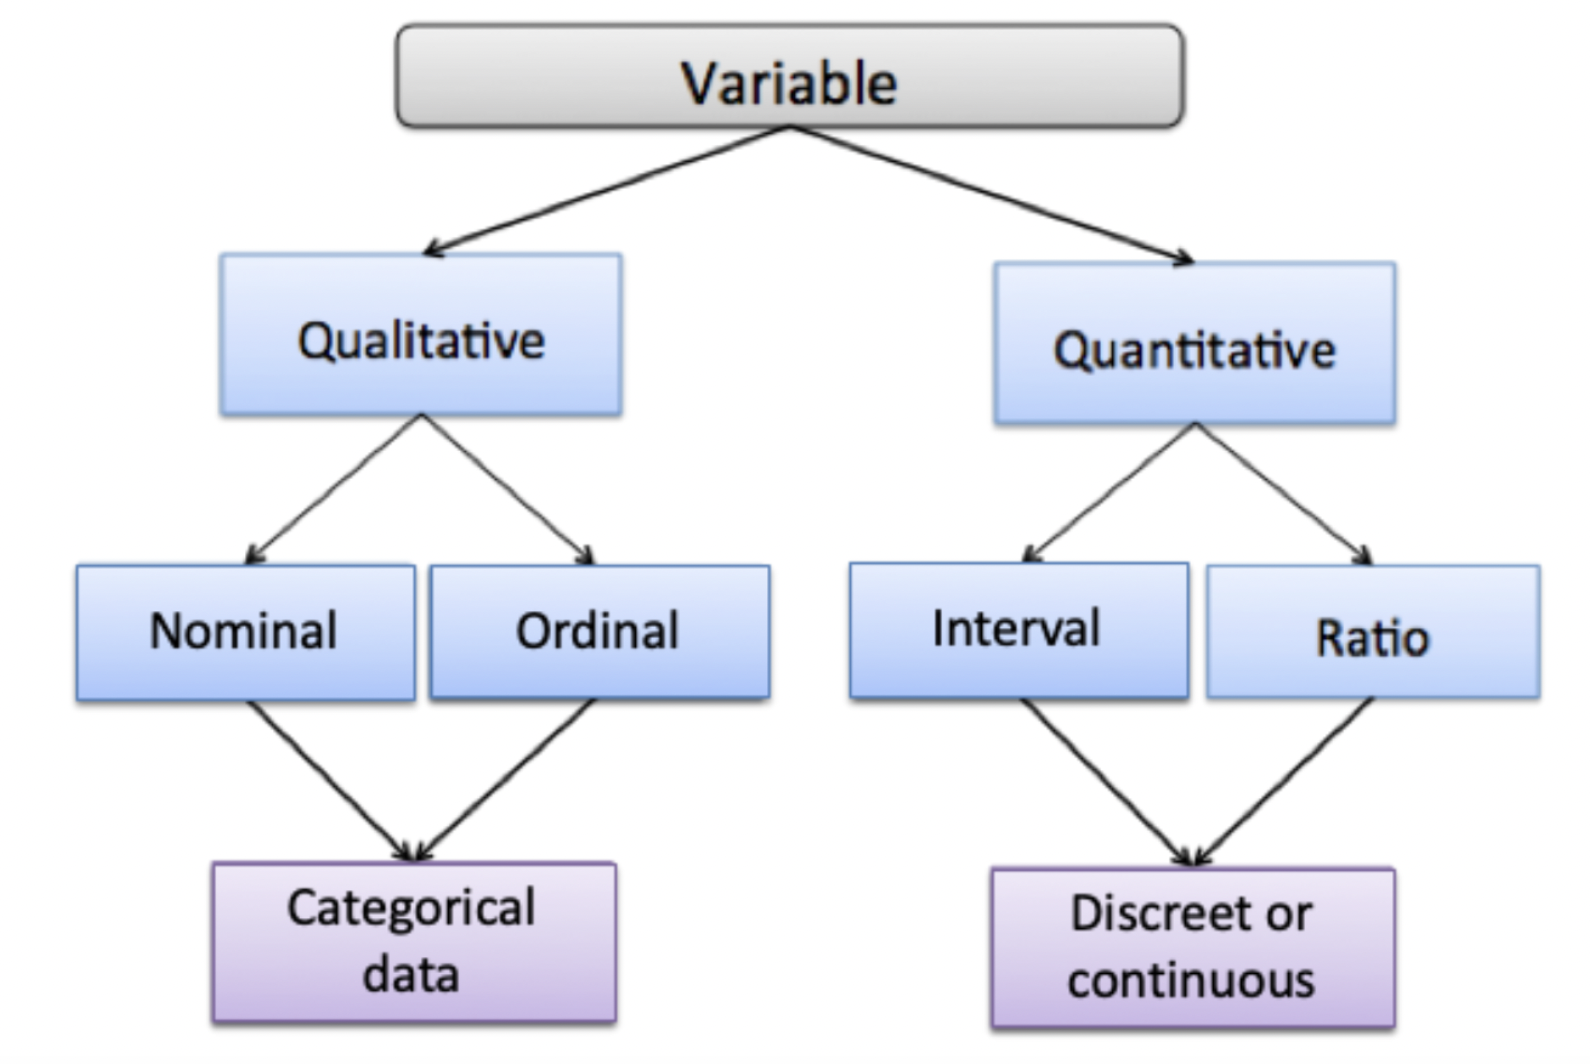
\includegraphics[scale=0.3]{p1.png}
    \caption{Variable Type}
    \label{}
\end{figure}\end{center}
\begin{enumerate}[a)]
    \item Nominal: Categories do not have a natural order. Ex. blood type, gender.
    \item Ordinal: Categories have a natural order. Ex. low/middle/high education level
    \item Interval: There is a numerical distance (difference between two different values is meaningful) between any two values.
    Ex. blood pressure level, 100 blood pressure doesn't mean the double degree of 50 pressure.
    \item Ratio: An interval variable where ratios are valid (presence of absolute zero, i.e. zero is meaningful). Ex. weight, 4g is double degree of 2g, distance run by an athlete.
\end{enumerate}
\subsection*{Levels of measurements}
A variable's level of measurement determines the statistical methods to be used for its analysis.
\begin{center}
    Variables hierarchy: Ratio $>$ Interval $>$ Ordinal $>$ Nominal
\end{center}
Statistical methods applied to variables at a lower level can be used with variables at a higher level, but the contrary is not true.

\section{Statistical Inference for Categorical Data}
There is a distribution $F(\beta)$ with p.d.f. (p.m.f.) $f(x\mid\beta)$, where $\beta$ a generic unknown parameter and $\hat{\beta}$ the parameter estimate.
\subsection{Maximum likelihood Estimation (MLE)}
Given a set of observations $\vec{x}=(x_1,...,x_n)$, the likelihood function of these observations with parameter $\beta$ is $l(\vec{x}\mid\beta)$. We want to find parameter $\hat{\beta}$ that maximizes the likelihood function,$$\hat{\beta}=\arg\max_{\beta} l(\vec{x}\mid\beta)$$
which is also equivalent to maximizing the logarithm of the likelihood function $L(\vec{x}\mid\beta) = \log(l(\vec{x}\mid\beta))$, $$\hat{\beta}=\arg\max_{\beta}L(\vec{x}\mid\beta)$$

\begin{definition}[score function]
    \normalfont
    The score function is $$u(\beta,\vec{x})=\nabla_{\beta} L(\vec{x}\mid \beta)=\frac{\nabla_{\beta} l(\vec{x}\mid \beta)}{l(\vec{x}\mid \beta)}$$
\end{definition}
\begin{lemma}[mean of score function]
    The mean of score function is $0$,
    $$\mathbb{E}_{\vec{x}}u(\beta,\vec{x})=0$$
\end{lemma}
\begin{proof}
    \begin{equation}
        \begin{aligned}
            \mathbb{E}_{\vec{x}}u(\beta,\vec{x})&=\int_{\vec{x}}l(\vec{x}\mid \beta)\frac{\nabla_{\beta} l(\vec{x}\mid \beta)}{l(\vec{x}\mid \beta)}d \vec{x}\\
            &=\int_{\vec{x}}\nabla_{\beta} l(\vec{x}\mid \beta)d \vec{x}\\
            &=\nabla_{\beta}\left(\int_{\vec{x}}l(\vec{x}\mid \beta)d \vec{x}\right)\\
            &=\nabla_{\beta}1=0
        \end{aligned}
        \nonumber
    \end{equation}
\end{proof}

\begin{lemma}[variance of score function]
    The variance of the score function is $$\textnormal{Var}_{\vec{x}}(u(\beta, \vec{x}))= \mathbb{E}_{\vec{x}}\left(u(\beta, \vec{x})u(\beta, \vec{x})^T\right)$$
\end{lemma}
\begin{proof}
    Prove by the zero mean.
\end{proof}

\begin{definition}[Fisher information]
    \normalfont
    The (Fisher) information is $$\iota(\beta)=-\mathbb{E}_{\vec{x}}\left[\nabla^2_\beta L(\vec{x}\mid\beta)\right]$$
\end{definition}
\begin{lemma}
    The Fisher information is equal to the variance of score function.
    $$\textnormal{Var}_{\vec{x}}(u(\beta, \vec{x}))=\mathbb{E}_{\vec{x}}\left(u(\beta,\vec{x})u(\beta,\vec{x})^T\right)=-\mathbb{E}_{\vec{x}}\left[\nabla^2_\beta L(\vec{x}\mid\beta)\right]=\iota(\beta)$$
\end{lemma}
\begin{proof}
    \begin{equation}
        \begin{aligned}
            \mathbb{E}_{\vec{x}}\left[\nabla^2_\beta L(\vec{x}\mid\beta)\right]=\mathbb{E}_{\vec{x}}\left(\frac{\partial \frac{\nabla_{\beta} l(\vec{x}\mid \beta)}{l(\vec{x}\mid \beta)}}{\partial \beta}\right)=\mathbb{E}_{\vec{x}}\left(\frac{\nabla^2_{\beta} l(\vec{x}\mid \beta)}{l(\vec{x}\mid \beta)}-\frac{\nabla_{\beta} l(\vec{x}\mid \beta)\nabla_{\beta} l(\vec{x}\mid \beta)^T}{(l(\vec{x}\mid \beta))^2} \right)
        \end{aligned}
        \nonumber
    \end{equation}
    where $\mathbb{E}_{\vec{x}}\left(\frac{\nabla^2_{\beta} l(\vec{x}\mid \beta)}{l(\vec{x}\mid \beta)}\right)=\int_{\vec{x}}l(\vec{x}\mid \beta)\frac{\nabla^2_{\beta} l(\vec{x}\mid \beta)}{l(\vec{x}\mid \beta)}d \vec{x}=\int_{\vec{x}}\nabla^2_{\beta} l(\vec{x}\mid \beta)d \vec{x}=\nabla^2_{\beta}\int_{\vec{x}} l(\vec{x}\mid \beta)d \vec{x}=\nabla^2_{\beta} 1=0$
    Hence, $$\mathbb{E}_{\vec{x}}\left[\nabla^2_\beta L(\vec{x}\mid\beta)\right]=-\mathbb{E}_{\vec{x}}\left(\frac{\nabla_{\beta} l(\vec{x}\mid \beta)\nabla_{\beta} l(\vec{x}\mid \beta)^T}{(l(\vec{x}\mid \beta))^2} \right)=-\mathbb{E}_{\vec{x}}\left(u(\beta,\vec{x})u(\beta,\vec{x})^T\right)$$
\end{proof}

\begin{proposition}
    When the sample $x$ is made up of i.i.d. observations, the covariance matrix of the maximum likelihood estimator $\hat{\beta}$ is approximately equal to the inverse of the information matrix. $$\textnormal{Cov}(\hat{\beta})\approx(\iota(\beta))^{-1}$$
\end{proposition}
Hence, the covariance matrix can be estimated as $(\iota(\hat{\beta}))^{-1}$. Similarly, \textit{SE} is estimated by $\sqrt{(\iota(\hat{\beta}))^{-1}}$.

\subsection{Likelihood Inference (Wald, Likelihood-Ratio, Score)}
We want to test
\begin{equation}
    \begin{aligned}
        H_0:\beta=\beta_0\quad\quad H_\alpha:\beta\neq \beta_0
    \end{aligned}
    \nonumber
\end{equation}
or form a confidence interval (CI) for $\beta$.

\begin{definition}[Wald Test]
    \normalfont
    The Wald statistic:
    \begin{equation}
        \begin{aligned}
            z_W=\frac{\hat{\beta}-\beta_0}{SE}=\frac{\hat{\beta}-\beta_0}{\sqrt{(\iota(\hat{\beta}))^{-1}}}
        \end{aligned}
        \nonumber
    \end{equation}
    where $\textit{SE}=\sqrt{(\iota(\hat{\beta}))^{-1}}$.\\
    Usually, as $n \rightarrow \infty$, $z_W \stackrel{d}{\longrightarrow} N(0,1)$ under $H_0:\beta=\beta_0$.
    \begin{enumerate}[(1)]
        \item We reject the $H_0$ if $|z_W|\geq z_{\frac{\alpha}{2}}$ for a \underline{two-sided level $\alpha$ test}.
        \item The \underline{$(1-\alpha)100\%$ Wald (confidence) interval} is $$\{\beta_0:|z_W|=\frac{|\hat{\beta}-\beta_0|}{SE}<z_{\frac{\alpha}{2}}\}=(\hat{\beta}-z_\frac{\alpha}{2}SE,\hat{\beta}+z_\frac{\alpha}{2}SE)$$
        \item The Wald test also has a \underline{chi-squared form}, using
        \begin{equation}
            \begin{aligned}
                z_W^2=\frac{(\hat{\beta}-\beta_0)^2}{(\iota(\hat{\beta}))^{-1}}\sim \chi_1^2\quad \textnormal{(under $H_0$)}
            \end{aligned}
            \nonumber
        \end{equation}
    \end{enumerate}
\end{definition}

\begin{definition}[Likelihood Ratio Test]
    \normalfont
    Let $$\Lambda=\frac{l(\vec{x}\mid\beta_0)}{l(\vec{x}\mid\hat{\beta})}$$
    where $l(\vec{x}\mid\hat{\beta})=\max_{\beta}l(\vec{x}\mid\beta)$, so the ratio $\Lambda\in [0,1]$.\\
    The \textbf{likelihood-ratio test (LRT) chi-squared statistic}:
    \begin{equation}
        \begin{aligned}
            -2\ln\Lambda=-2\left(L(\beta_0)-L(\hat{\beta})\right)
        \end{aligned}
        \nonumber
    \end{equation}
    It has an approximate $\chi_1^2$ distribution under $H_0 : \beta = \beta_0$, and otherwise tends to be larger.
    \begin{enumerate}[(1)]
        \item Thus, reject $H_0$ if $$-2\ln\Lambda\geq\chi_1^2(\alpha)$$
        \item The \underline{$(1-\alpha)100\%$ likelihood-ratio (confidence) interval} is $$\{\beta_0:-2\ln\Lambda=-2\left(L(\beta_0)-L(\hat{\beta})\right)<\chi_1^2(\alpha)\}$$
        Unlike Wald, this interval is \underline{not degenerate}. (i.e., For general case, the interval does not have an explicit form.)
    \end{enumerate}
\end{definition}

\begin{definition}[Score Test]
    \normalfont
    The \textbf{score statistic}: $$z_S=\frac{u(\beta_0)}{\sqrt{\iota(\beta_0)}}$$
    As $n \rightarrow \infty$, $z_S \stackrel{d}{\longrightarrow} N(0,1)$ under $H_0:\beta=\beta_0$. Otherwise, it tends to be further from zero.
    \begin{enumerate}[(1)]
        \item Thus, reject $H_0$ if $|z_S|\geq z_{\frac{\alpha}{2}}$ for a \underline{two-sided level $\alpha$ test}.
        \item The \underline{$(1-\alpha)100\%$ score (confidence) interval} is $$\{\beta_0:|z_S|=\frac{|u(\beta_0)|}{\sqrt{\iota(\beta_0)}}<z_{\frac{\alpha}{2}}\}$$
        Unlike Wald, it is \underline{not degenerate} for some distributions.
        \item There is also a chi-squared form:
        \begin{equation}
            \begin{aligned}
                z_S^2=\frac{u(\beta_0)^2}{\iota(\beta_0)}\sim \chi_1^2\quad \textnormal{(under $H_0$)}
            \end{aligned}
            \nonumber
        \end{equation}
    \end{enumerate}
\end{definition}
We can also use P-value to measure the probability of the statistic is more extreme under the $H_0$. We can reject $H_0$ if the P-value is $\leq\alpha$.

All three kinds tend to be “asymptotically equivalent” as $n \rightarrow \infty$. For smaller $n$, the \underline{likelihood-ratio} and \underline{score} methods are preferred.

\chapter{Association in Contingency Tables}
\section{Association in Two-Way Contingency Tables}
Consider joint observations of two categorical variables: $X$ with $I$ categories, $Y$ with $J$ categories.

We can summarize data in an $I \times J$ \textbf{contingency table}:
\begin{table}[htbp]
    \centering
    \begin{tabular}{lllll}
        &&&$Y$&\\
        &&1&$\cdots$&J\\
        \cline{3-5}
        & \multicolumn{1}{l|}{$1$} & \multicolumn{1}{l|}{} & \multicolumn{1}{l|}{} & \multicolumn{1}{l|}{} \\
        \cline{3-5}
        $X$ &\multicolumn{1}{l|}{$\vdots$}  & \multicolumn{1}{l|}{} & \multicolumn{1}{l|}{} & \multicolumn{1}{l|}{} \\ \cline{3-5}
        & \multicolumn{1}{l|}{$I$} & \multicolumn{1}{l|}{} & \multicolumn{1}{l|}{} & \multicolumn{1}{l|}{} \\ \cline{3-5}
    \end{tabular}
\end{table}\\
Each \textbf{cell} contains a count $n_{ij}$.

\subsection{Distribution}
If both $X$ and $Y$ are random, let $$\pi_{ij}=P(X\text{ in row }i, Y\text{ in col }j)$$
be the \textbf{joint} distribution of $X$ and $Y$.

The \textbf{marginal} distribution of $X$ is defined by $$\pi_{i+}=P(X\text{ in row }i)$$
and similarly for $Y$:
$$\pi_{+j}=P(Y\text{ in col }j)$$

The \textbf{conditional} distribution of $Y$ given that $X$ is in row $i$ is defined by
$$\pi_{j\mid i}=P(Y\text{ in col }j\mid X\text{ in row }i)=\frac{\pi_{ij}}{\pi_{i+}}$$

\subsection{Descriptive Statistics}
Let $n_{ij}=\textit{count in row $i$ and col $j$}$ and $n=\sum_i\sum_jn_{ij}$.\\
The \textbf{margins} of the table:
$$n_{i+}=\sum_jn_{ij},\quad n_{+j}=\sum_in_{ij}$$
\subsubsection*{Natural Estimation}
\begin{enumerate}
    \item Natural estimate of $\pi_{ij}$: $\hat{\pi}_{ij}=\frac{n_{ij}}{n}$
    \item Similarly marginals: $\hat{\pi}_{i+}=\sum_j \hat{\pi}_{ij}=\frac{n_{i+}}{n};\ \hat{\pi}_{+j}=\sum_i p_{ij}=\frac{n_{+j}}{n}$
    \item And conditionals: $\hat{\pi}_{j\mid i}=\frac{\hat{\pi}_{ij}}{\hat{\pi}_{i+}}=\frac{n_{ij}}{n_{i+}}$
\end{enumerate}

\subsection{Sampling Models (Examples)}
Possible joint distributions for counts in $I \times J$ table:
\begin{enumerate}
    \item \underline{Poisson (random total)}: $Y_{ij} =\text{count in cell } (i,j)$,
    $$Y_{ij}\sim \text{Poisson}(\mu_{ij})$$
    and the $Y_{ij}$s are independent.
    \item \underline{Multinomial (fixed total $n$):} $N_{ij} = \text{count in cell } (i,j)$, $$\{N_{ij}\}\sim \text{multinomial}(n,\{\pi_{ij}\})$$
    \item \underline{Independent Multinomial}: Assume $n_{i+}$ (row totals $n_i$) are fixed,
    \begin{equation}
        \begin{aligned}
            \left.\begin{matrix}
                \{N_{1j}\}_{j=1}^J\sim \text{multinomial}(n_1,\{\pi_{j\mid 1}\}_{j=1}^J)\\
                \vdots\\
                \{N_{Ij}\}_{j=1}^J\sim \text{multinomial}(n_I,\{\pi_{j\mid I}\}_{j=1}^J)\\
            \end{matrix}\right\}
        \end{aligned}
        \nonumber
    \end{equation}
    (When $J = 2$, this is \underline{independent binomial sampling}, for which we may just write $\pi_i$ for $\{\pi_{1\mid i},\pi_{2\mid i}\}$.)
\end{enumerate}


\subsection{Independent / Homogeneity}
\begin{definition}[independent]
    \normalfont
    If both $X$ and $Y$ are \underline{random}, they are \textbf{independent} if $$\pi_{ij}=\pi_{i+}\pi_{+j},\ \forall i,j$$
    which implies $\pi_{j\mid i}=\frac{\pi_{i+}\pi_{+j}}{\pi_{i+}}=\pi_{+j},\forall i,j$. That is, $\pi_{j\mid i}$ doesn't depend on $i$ and is the same as the marginal distribution of $Y$. (Intuitively, knowing $X$ tells nothing about $Y$.)
\end{definition}
\begin{definition}[homogeneity]
    \normalfont
    Even if $X$ is \underline{not really random}, the condition that $\pi_{j\mid i}=\pi_{+j},\forall i,j$ is called \textbf{homogeneity}. This might still be relevant in a situation where $X$ is deliberately chosen and $Y$ is observed as a response.
\end{definition}



\subsection{Measuring Inhomogeneity}
\begin{table}[htbp]
    \centering
    \begin{tabular}{rllll}
        \cline{2-5}
        \multicolumn{1}{r|}{\multirow{2}{*}{}} & \multicolumn{2}{l|}{$n_{11}$} & \multicolumn{2}{l|}{$n_{12}$} \\ \cline{2-5} 
        \multicolumn{1}{r|}{}                   & \multicolumn{2}{l|}{$n_{21}$} & \multicolumn{2}{l|}{$n_{22}$} \\ \cline{2-5}
        \multicolumn{1}{l}{}                    &             &             &             &
    \end{tabular}\\
    \begin{tabular}{rllll}
        \cline{2-5}
        \multicolumn{1}{r|}{\multirow{2}{*}{}} & \multicolumn{2}{l|}{$Y_1$} & \multicolumn{2}{l|}{$n_1-Y_1$} \\ \cline{2-5} 
        \multicolumn{1}{r|}{}                   & \multicolumn{2}{l|}{$Y_2$} & \multicolumn{2}{l|}{$n_2-Y_2$} \\ \cline{2-5}
        \multicolumn{1}{l}{}                    &             &             &             &
    \end{tabular}\\
    where $Y_i\sim$ indep. binomial$(n_i,\pi_i)$. This regards row totals as fixed.
\end{table}
Homogeneity is the condition $\pi_1 = \pi_2$. We can measure inhomogeneity by three different measures:
\begin{enumerate}
    \item \textbf{difference of proportions}: $$\pi_1-\pi_2$$
    The estimation is $$\hat{\pi}_1-\hat{\pi}_2=\frac{y_1}{n_1}-\frac{y_2}{n_2}$$
    The approx $(1-\alpha)100\%$ confidence interval is:
    \begin{equation}
        \begin{aligned}
            \hat{\pi}_1-\hat{\pi}_2\pm z_{\frac{\alpha}{2}}\sqrt{\frac{\hat{\pi}_1(1-\hat{\pi}_1)}{n_1}+\frac{\hat{\pi}_2(1-\hat{\pi}_2)}{n_2}}
        \end{aligned}
        \nonumber
    \end{equation}
    (Problematic if $\pi_1$ and $\pi_2$ are near $0$ or $1$.)
    \item \textbf{relative risk}: $$RR=\frac{\pi_1}{\pi_2}$$
    The estimation is $$r=\frac{\hat{\pi}_1}{\hat{\pi}_2}=\frac{y_1/n_1}{y_2/n_2}$$
    The approx $(1-\alpha)100\%$ confidence interval of $\ln RR$ is:
    \begin{equation}
        \begin{aligned}
            \ln r\pm z_{\frac{\alpha}{2}}\sqrt{\frac{1-\hat{\pi}_1}{y_1}+\frac{1-\hat{\pi}_2}{y_2}}
        \end{aligned}
        \nonumber
    \end{equation}
    \item \textbf{odds ratio}: $$\theta=\frac{\pi_1/(1-\pi_1)}{\pi_2/(1-\pi_2)}$$
    When $\theta=1$, we can say there is no association.\\
    The \textbf{odds} for a probability $\pi$ is $\Omega=\frac{\pi}{1-\pi}$. Note $\pi=\frac{\Omega}{1+\Omega}$.\\
    (In the multinomial model: $\theta=\frac{\pi_{11}\pi_{22}}{\pi_{12}\pi_{21}}$ ("cross-product ratio"); in Poisson model: $\theta=\frac{\mu_{11}\mu_{22}}{\mu_{12}\mu_{21}}$)\\
    The usual (unrestricted) estimates $$\hat{\theta}=\frac{n_{11}n_{22}}{n_{12}n_{21}}$$
    The approx $(1-\alpha)100\%$ confidence interval for $\ln\theta$ is
    \begin{equation}
        \begin{aligned}
            \ln\hat{\theta}\pm z_{\frac{\alpha}{2}}\sqrt{\frac{1}{n_{11}}+\frac{1}{n_{12}}+\frac{1}{n_{21}}+\frac{1}{n_{22}}}
        \end{aligned}
        \nonumber
    \end{equation}
    Useful properties of odds ratio:
    \begin{enumerate}[(1)]
        \item Interchanging rows (or cols) changes $\theta$ to $\frac{1}{\theta}$.
        \item Interchanging $X$ and $Y$ doesn't change $\theta$.
        \item Multiplying a row (or col) by a factor doesn't change $\hat{\theta}$.
        \item Relationship to relative risk: $\theta=RR\cdot\frac{1-\pi_2}{1-\pi_1}$. ($\theta$ and $RR$ are similar if both $\pi_1$ and $\pi_2$ are small.)
    \end{enumerate}
\end{enumerate}
\subsection{Delta Method}
It is easy to obtain approximate CI for a mean based on a sample mean by using the Central Limit Theorem and a consistent estimate of standard error.

But the log Odds Ratio and log Relative Risk are transformed means. How were their CI's derived? And why take logs?

Suppose a statistic $T_n$ and parameter $\theta$ such that
$$
\sqrt{n}\left(T_n-\theta\right) \underset{n \rightarrow \infty}{\stackrel{d}{\longrightarrow}} N\left(0, \sigma^2\right)
$$
(e.g. $T_n$ might be a sample mean from a sample of size $n$ with population mean $\theta$ and variance $\sigma^2$)

We want a CI for $g(\theta)$, for some smooth $g$.

The Taylor expand at $T_n$ is
\begin{equation}
    \begin{aligned}
        %g(T_n)\approx g(\theta)+g'(\theta)(T_n-\theta)
        g(\theta)\approx g(T_n)+g'(T_n)(\theta-T_n)
    \end{aligned}
    \nonumber
\end{equation}
So,
\begin{equation}
    \begin{aligned}
        \sqrt{n}(g(T_n)-g(\theta))\approx g'(T_n)\sqrt{n}(T_n-\theta)\underset{n \rightarrow \infty}{\stackrel{d}{\longrightarrow}} N\left(0, (g'(T_n))^2\sigma^2\right)
    \end{aligned}
    \nonumber
\end{equation}
(This is useful only if $g'(T_n)\neq 0$)
Hence, when $n$ is large
\begin{equation}
    \begin{aligned}
        \sqrt{n}\frac{g(T_n)-g(\theta)}{|g'(T_n)|\sigma} \quad \dot{\sim}\quad  N(0,1)
    \end{aligned}
    \nonumber
\end{equation}
which suggests this approximate CI for $g(\theta)$:
\begin{equation}
    \begin{aligned}
        g(T_n)\pm z_{\frac{\alpha}{2}}\frac{|g'(T_n)|\sigma}{\sqrt{n}}
    \end{aligned}
    \nonumber
\end{equation}



\subsection{Testing Independence by Residuals: $X^2$ Test (Pearson)}
Let $\mu_{ij}=\mathbb{E}(N_{ij})=n\pi_{ij}$. Under $H_0:\pi_{ij}=\pi_{i+}\pi_{+j},\ \forall i,j$
\begin{equation}
    \begin{aligned}
        \mu_{ij}=n\pi_{ij}=n\pi_{i+}\pi_{+j}
    \end{aligned}
    \nonumber
\end{equation}
Under $H_0$, can show the MLEs are
\begin{equation}
    \begin{aligned}
        \hat{\mu}_{ij}=n\hat{\pi}_{i+}\hat{\pi}_{+j}=n\left(\frac{n_{i+}}{n}\right)\left(\frac{n_{+j}}{n}\right)=\frac{n_{i+}n_{+j}}{n}
    \end{aligned}
    \nonumber
\end{equation}
(assuming no empty rows or cols)\\
\textbf{Residuals:}
\begin{enumerate}
    \item Raw: $n_{ij}-\hat{\mu}_{ij}$
    \item Pearson: $e_{ij}=\frac{n_{ij}-\hat{\mu}_{ij}}{\sqrt{\hat{\mu}_{ij}}}$. $X^2=\sum_i\sum_j e_{ij}^2$.
    \item Standardized: $r_{ij}=\frac{n_{ij}-\hat{\mu}_{ij}}{\sqrt{\hat{\mu}_{ij}(1-\hat{\pi}_{i+})(1-\hat{\pi}_{+j})}}$
\end{enumerate}
\textbf{Usage:} Look for Pearson or standardized residuals with absolute value \textit{exceeding 2 or 3}. These suggest the reason for significant dependence.

\textbf{Remark:} Under independence, both Pearson and standardized residuals are asymp. normal, but only standardized has asymp. variance equal to 1.

\begin{definition}[$X^2$ Test: Pearson $\chi^2$ Test (Score Test)]
    \normalfont
    $$X^2=\sum_{i j} \frac{\left(n_{i j}-\hat{\mu}_{i j}\right)^2}{\hat{\mu}_{i j}} \quad \underset{H_0}{\dot{\sim}}\quad \chi_{(I-1)(J-1)}^2$$
    Note:
    $$
    \begin{aligned}
    (I-1)(J-1) & =(I J-1)-((I-1)+(J-1)) \\
    & =\text { total \# params. }-\# \text { params. under } H_0
    \end{aligned}
    $$
    Reject $H_0$ if
    $$
    X^2>\chi_{(I-1)(J-1)}^2(\alpha)
    $$
    (or use $P$-value)
\end{definition}
\begin{example}
    Testing independence is equivalent to testing homogeneity in the indep. binomial model:
    $$
    H_0: \pi_1=\pi_2
    $$
    Can show
    $$
    X^2=z^2
    $$
    where
    $$
    z=\frac{\hat{\pi}_1-\hat{\pi}_2}{\sqrt{\hat{\pi}(1-\hat{\pi})\left(1 / n_1+1 / n_2\right)}} \quad \hat{\pi}=\frac{y_1+y_2}{n_1+n_2}
    $$
\end{example}

\subsection{Testing Independence: $G^2$ Test (Likelihood Ratio)}
\begin{definition}[$G^2$ Test: Likelihood Ratio $\chi^2$ Test]
    \normalfont
    $$G^2=2\sum_{i j}n_{ij} \ln \frac{n_{i j}}{\hat{\mu}_{i j}} \quad \underset{H_0}{\dot{\sim}}\quad \chi_{(I-1)(J-1)}^2$$
    Reject $H_0$ if
    $$G^2>\chi_{(I-1)(J-1)}^2(\alpha)$$
    (or use $P$-value)\\
    (Convention: $0 \ln 0 = 0$)
\end{definition}
\textbf{Comparison:}
\begin{enumerate}
    \item $X^2$ and $G^2$ are asymptotically equivalent under $H_0$
    \item The $X^2$ tends to be better.
\end{enumerate}
\textbf{Remark:} The $X^2$ and $G^2$ tests are not necessarily compatible with the Wald CIs. For example,
\begin{center}
    reject $H_0$ $\nLeftrightarrow$  odds ratio $\theta =\frac{\pi_1/(1-\pi_1)}{\pi_2/(1-\pi_2)}= 1$ not in Wald CI
\end{center}

\subsection{Testing Independence: Fisher's Exact Test}
When cell counts are small, the $X^2$ and $G^2$ independence tests are not recommended: The $\chi^2$ approximations are poor. In this section we introduce a \textit{Fisher's Exact Test}.

Consider a $2 \times 2$ table with row and col totals fixed:
$$
\begin{array}{c|c|c|c}
\multicolumn{1}{r}{} &\multicolumn{2}{c}{Y} \\
\cline { 2 - 3 }
\multicolumn{1}{r|}{\multirow{2}{*}{$X$}} & N_{11} & N_{12} & n_{1+} \\
\cline { 2 - 3 } 
\multicolumn{1}{r|}{} & N_{21} & N_{22} & n_{2+} \\
\cline { 2 - 3 } \multicolumn{1}{c}{}&\multicolumn{1}{c}{n_{+1}}&\multicolumn{1}{c}{n_{+2}}&\multicolumn{1}{c}{n}
\end{array}
$$
\textbf{Note:} \underline{Any cell count, say $N_{11}$, determines the whole table.}

Can show that, under $H_0$ : independence, $N_{11}$ is (conditionally) hypergeometric:
$$
\mathrm{P}_{H_0}\left(N_{11}=t\right)=\frac{\begin{pmatrix}
    n_{1+} \\
    t
\end{pmatrix}\begin{pmatrix}
    n_{2+}\\
    n_{+1}-t
\end{pmatrix}}{\begin{pmatrix}
    n \\
    n_{+1}
\end{pmatrix}}
$$
In terms of odds ratio $\theta=\frac{\pi_1/(1-\pi_1)}{\pi_2/(1-\pi_2)}$, independence is $$H_0:\theta=1$$
Possible alternatives:
\begin{equation}
    \begin{aligned}
        H_\alpha:\theta>1 \quad &\Rightarrow\quad N_{11} \textnormal{ tends larger}\\
        H_\alpha:\theta<1 \quad &\Rightarrow\quad N_{11} \textnormal{ tends smaller}\\
        H_\alpha:\theta\neq 1 \quad &\Rightarrow\quad N_{11} \textnormal{ tends larger or smaller}
    \end{aligned}
    \nonumber
\end{equation}
For $H_\alpha:\theta>1$, the (one-sided) $p$-value is $\mathrm{P}_{H_0}\left(N_{11}\geq t_0\right)$, where $t_0=n_{11}$ is the observed value of $N_{11}$.

\textbf{Remarks:} Could use mid $p$-values instead; Implemented in R function fisher.test(); Can be extended to $I \times J$ tables (with some computational difficulty).


\section{Conditional Association in Three-Way Tables}
Add a third categorical variable $Z$.
\begin{example}
    Is a drug more effective at curing a disease among younger patients than among older?
    $X=$ drug or placebo; $Y=$ disease cured or not; $Z=$ age group (young, old).
\end{example}
\subsection{Conditional Association}
$Z$ may be called a \textbf{stratification variable}. We are interested in the distribution of $(X, Y)$ \textit{conditional} on $Z$.

\begin{definition}[partial table]
    \normalfont
    Each $Z$ category defines a \textbf{partial table} for $X$ and $Y$.
\end{definition}
\begin{example}
    When $Z = 1, 2$ and $X , Y$ are binary ($2\times 2 \times 2$ table):
    \begin{table}[htbp]
        \centering
        $Z=1:$
        \begin{tabular}{rllll}
            \multicolumn{1}{c}{}                    & \multicolumn{4}{c}{$Y$}                                 \\ \cline{2-5} 
            \multicolumn{1}{r|}{\multirow{2}{*}{$X$}} & \multicolumn{2}{l|}{$n_{111}$} & \multicolumn{2}{l|}{$n_{121}$} \\ \cline{2-5} 
            \multicolumn{1}{r|}{}                   & \multicolumn{2}{l|}{$n_{211}$} & \multicolumn{2}{l|}{$n_{221}$} \\ \cline{2-5}
            \multicolumn{1}{l}{}                    &             &             &             &
        \end{tabular}\quad\quad
        $Z=2:$
        \begin{tabular}{rllll}
            \multicolumn{1}{c}{}                    & \multicolumn{4}{c}{$Y$}                                 \\ \cline{2-5} 
            \multicolumn{1}{r|}{\multirow{2}{*}{$X$}} & \multicolumn{2}{l|}{$n_{112}$} & \multicolumn{2}{l|}{$n_{122}$} \\ \cline{2-5} 
            \multicolumn{1}{r|}{}                   & \multicolumn{2}{l|}{$n_{212}$} & \multicolumn{2}{l|}{$n_{222}$} \\ \cline{2-5}
            \multicolumn{1}{l}{}                    &             &             &             &
        \end{tabular}\\
        These represent \textbf{conditional associations}.
    \end{table}\\
\end{example}

\begin{definition}[marginal table]
    \normalfont
    The \textbf{marginal table} sums the partial tables:
\end{definition}
\begin{table}[htbp]
    \centering
    \begin{tabular}{rllll}
        \multicolumn{1}{c}{}& \multicolumn{4}{c}{$Y$}\\
        \cline{2-5}
        \multicolumn{1}{r|}{\multirow{2}{*}{$X$}}&\multicolumn{2}{l|}{$n_{11+}$}&\multicolumn{2}{l|}{$n_{12+}$}\\
        \cline{2-5}
        \multicolumn{1}{r|}{}&\multicolumn{2}{l|}{$n_{21+}$}&\multicolumn{2}{l|}{$n_{22+}$}\\
        \cline{2-5}
        \multicolumn{1}{l}{}&&&&
    \end{tabular}\\
    This represents the \textbf{marginal association} (ignoring $Z$).
\end{table}
In general, let $\mu_{ijk}=\textit{ expected count in row i, col j, table k}$.\\
The \textbf{conditional odds ratios},
\begin{equation}
    \begin{aligned}
        \theta_{XY(k)}=\frac{\mu_{11k}\mu_{22k}}{\mu_{12k}\mu_{21k}}
    \end{aligned}
    \nonumber
\end{equation}
which are estimated by
\begin{equation}
    \begin{aligned}
        \hat{\theta}_{XY(k)}=\frac{n_{11k}n_{22k}}{n_{12k}n_{21k}}
    \end{aligned}
    \nonumber
\end{equation}
The \textbf{marginal odds ratio}
\begin{equation}
    \begin{aligned}
        \theta_{XY}=\frac{\mu_{11+}\mu_{22+}}{\mu_{12+}\mu_{21+}}
    \end{aligned}
    \nonumber
\end{equation}
is estimated from the marginal table.

\subsection{Simpson's Paradox}
Some counter-intuitive but possible situations:
\begin{enumerate}
    \item There are conditional associations ($\theta_{XY(k)} \neq 1$) but no marginal
    association ($\theta_{XY} = 1$)
    \item There is a marginal association ($\theta_{XY} \neq 1$) but no conditional associations ($\theta_{XY(k)} = 1$)
    \item \textbf{Simpson's paradox}: The conditional associations are in the opposite direction from the marginal, e.g. $\theta_{XY(k)}>1,\theta_{XY}<1$
    \begin{center}\begin{figure}[htbp]
        \centering
        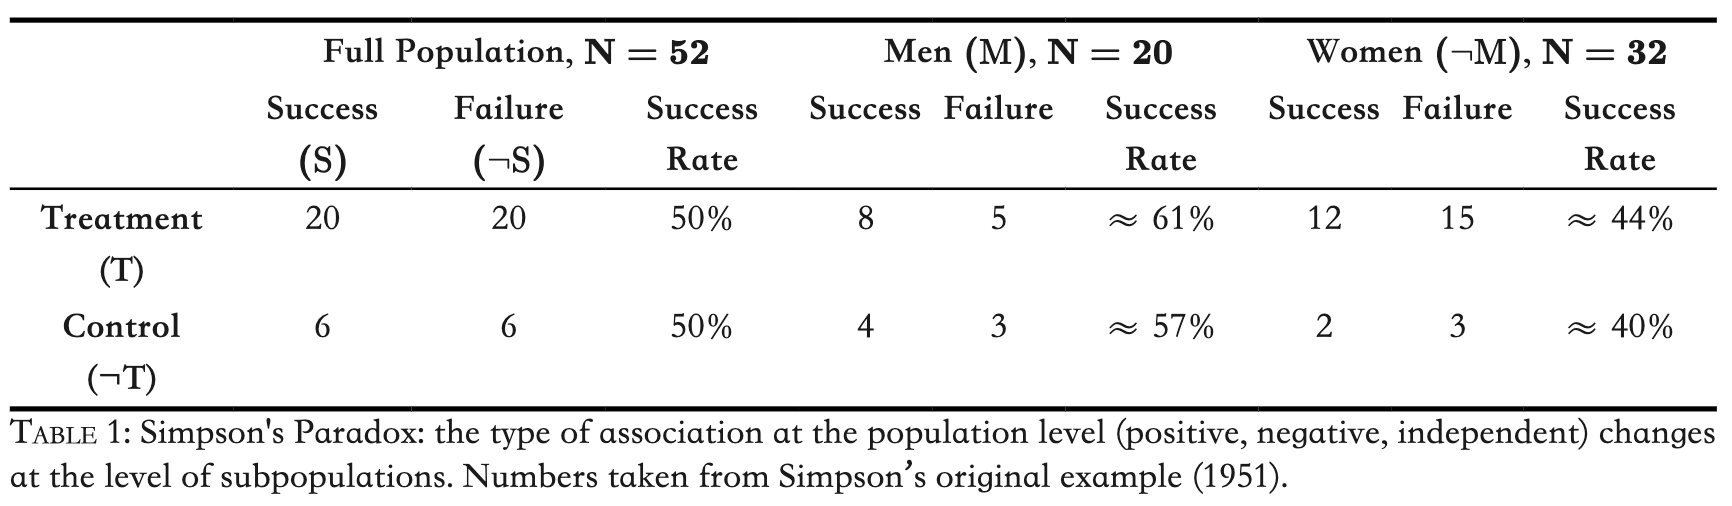
\includegraphics[scale=0.2]{Simpson's Paradox.png}
        \caption{Simpson's paradox}
        \label{}
    \end{figure}\end{center}
\end{enumerate}

\subsection{Conditional Independence, Marginal Independence}
\begin{definition}[conditionally independent given $Z$, marginal independent]
    \normalfont
    We also call $X$ and $Y$ are \textbf{conditionally independent given $Z = k$} if $\theta_{XY(k)}=1$. If this is true for all $k$, $X$ and $Y$ are \textbf{conditionally independent given $Z$}. Not the same to "$X$ and $Y$ are \textbf{marginal independent} if $\theta_{XY}=1$".
\end{definition}

\begin{proposition}
    For \underline{multinomial sampling}, can show that conditional independence is
    \begin{equation}
        \begin{aligned}
            \pi_{ijk}=\frac{\pi_{i+k}\pi_{+jk}}{\pi_{++k}},\quad \forall i,j,k
        \end{aligned}
        \nonumber
    \end{equation}
\end{proposition}

\subsection{Homogeneous Association}
\begin{definition}
    \normalfont
    Let $Z$ have $K$ categories. $X$ and $Y$ have \textbf{homogeneous association} over $Z$ if
    \begin{equation}
        \begin{aligned}
            \theta_{XY(1)}=\theta_{XY(2)}=\cdots=\theta_{XY(K)}
        \end{aligned}
        \nonumber
    \end{equation}
    (Conditional independence is a special case.)
\end{definition}

\chapter{Generalized Linear Models}
\section{Introduction}
A linear model $Y=\alpha+\sum_{i=1}^p \beta_i x_i +\varepsilon$ is usually not appropriate if $Y$ is binary or a count.

\subsection{Definition}
We seek to model independent observations $Y_1,...,Y_n$ of a \textbf{response variable}, in terms of corresponding vectors $\vec{x}_i=(x_{i1},...,x_{ip}),i=1,...,n$ of values of $p$ \textbf{explanatory variables}.

\begin{enumerate}[(1)]
    \item \textbf{\underline{Random component:}} density of $Y_i$ from a \textbf{natural exponential family} $$f(y_i;\theta_i)=a(\theta_i)b(y_i)\textnormal{exp}(y_i Q(\theta_i))$$
    where $Q(\theta_i)$ is the \textbf{natural parameter}.\\
    (\textbf{Fact:} Since $Y_i$ is from a natural exponential family, its distribution is completely determined by its mean $\mu_i$. In particular, $\textnormal{Var}(Y_i)$ is a function of $\mu_i$.)
    \item \textbf{\underline{Systematic component:}} the \textbf{linear predictor}
    $$\eta_i = \alpha+\beta_1 x_{i1}+\cdots +\beta_p x_{ip}$$
    with parameters $\alpha,\beta_1,...\beta_p$ (\textbf{coefficients})\\
    $Y_i$ will depend on $\vec{x}_i$ only through $\eta_i$.
    \item \textbf{\underline{Link function:}} monotonic, differentiable $g$ such that $g(\mu_i)=\eta_i$, that is
    $$g(\mu_i)=\alpha+\beta_1 x_{i1}+\cdots +\beta_p x_{ip}\quad \textnormal{ where }\mu_i=\mathbb{E}(Y_i)$$
    (Note: Ordinary linear models use the identity link: $g(\mu)=\mu$, which means $\mu_i=\alpha+\beta_1 x_{i1}+\cdots +\beta_p x_{ip}$.)
    \begin{definition}[Canonical Link]
        \normalfont
        The \textbf{canonical link} satisfies $$Q(\theta_i)=g(\mu_i)=\alpha+\beta_1 x_{i1}+\cdots +\beta_p x_{ip}$$
    \end{definition}
\end{enumerate}

Let $F$ be a continuous and invertible c.d.f. on the real line.
A reasonable link might be
$$
g(\pi)=F^{-1}(\pi)
$$
since it transforms interval $(0,1)$ to the whole real line.
\begin{definition}[Probit Regression]
    \normalfont
    Using the c.d.f. $\Phi$ for a standard normal is called \textbf{probit regression}.
\end{definition}


\subsection{Fitting GLMs}
Usually by maximum likelihood: find
$$
\hat{\alpha}, \hat{\beta}_1, \ldots, \hat{\beta}_p
$$
maximizing
$$
\prod_{i=1}^n f\left(y_i ; \theta_i\right)
$$
Explicit solutions exist only in special cases, so need numerical methods: e.g. Newton-Raphson, Fisher Scoring.

\section{Binary and Binomial Responses}
\subsection{Binary Regression}
\begin{example}[ (Binary Regression)]
    \begin{equation}
        \begin{aligned}
        Y_i & \sim \operatorname{Bernoulli}\left(\pi_i\right) \quad\left(\theta_i=\pi_i\right) \\
        f\left(y_i ; \pi_i\right) & = \left\{\begin{matrix}
            1-\pi_i & y_i=0 \\
            \pi_i & y_i=1
        \end{matrix}\right.\\
        & =\pi_i^{y_i}\left(1-\pi_i\right)^{1-y_i} \\
        & =\left(1-\pi_i\right)\left(\frac{\pi_i}{1-\pi_i}\right)^{y_i} \\
        & =\left(1-\pi_i\right) \exp \left(y_i \ln \left(\frac{\pi_i}{1-\pi_i}\right)\right)
        \end{aligned}
        \nonumber
    \end{equation}
    So $a(\pi)=1-\pi, b(y)=1$, and
    $$
    Q(\pi)=\ln \left(\frac{\pi}{1-\pi}\right)=\operatorname{logit}(\pi)
    $$
    The natural parameter is the \textbf{log odds}.\\
    Note: $\mu_i=E\left(Y_i\right)=\pi_i$. Hence, we can write $\pi_i(\vec{x}_i)$ as a response to
    \begin{enumerate}[$\bullet$]
        \item \textbf{Identity Link:} $$\pi(\vec{x}_i)=\alpha+\beta_1 x_{i1} + \cdots + \beta_p x_{ip}$$
        \item \textbf{Log Link:} $$\ln (\pi(\vec{x}_i))=\alpha+\beta_1 x_{i1} + \cdots + \beta_p x_{ip}$$
        \item \textbf{Canonical link: (logistic regression)}
        $$
        \operatorname{logit}(\pi(\vec{x}_i))=\alpha+\beta_1 x_{i1} + \cdots + \beta_p x_{ip}
        $$
        Specifically, when $p=1$,
        \begin{equation}
            \begin{aligned}
                \operatorname{logit}(\pi(x))=\alpha+\beta x\quad &\Leftrightarrow\quad \textnormal{odds}(\pi(x))=e^{\alpha+\beta x}\\
                &\Leftrightarrow\quad \pi(x)=\frac{e^{\alpha+\beta x}}{1+e^{\alpha+\beta x}}
            \end{aligned}
            \nonumber
        \end{equation}
        \begin{center}\begin{figure}[htbp]
            \centering
            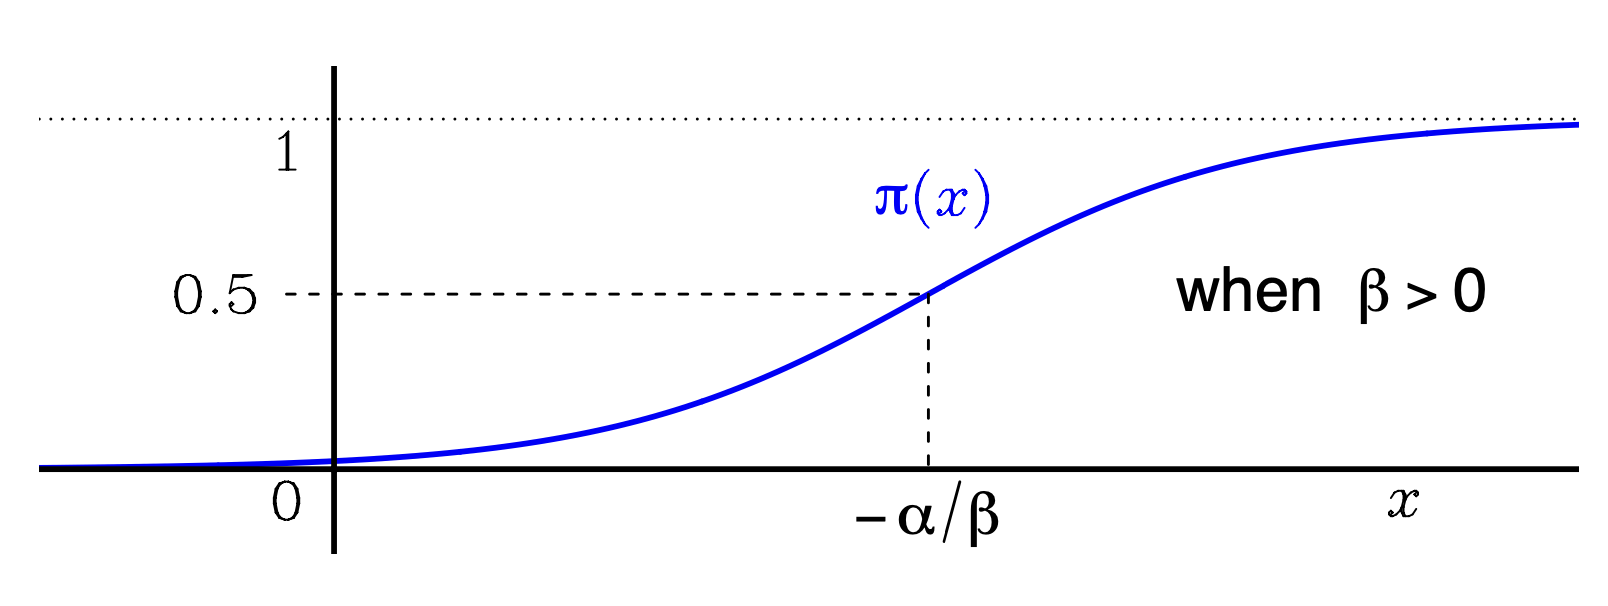
\includegraphics[scale=0.18]{logit.png}
            \caption{$\pi(x)=\frac{e^{\alpha+\beta x}}{1+e^{\alpha+\beta x}}$}
            \label{}
        \end{figure}\end{center}
    \end{enumerate}
\end{example}

\subsection{Grouped Data: Binomial Response}
If several observations have the same $\vec{x}$ ("replications"), then they have the same $\pi(\vec{x})$.

Summing binary (0/1) observations with the same $\vec{x}$ gives \textbf{grouped} data:
$$
Y_i \sim \operatorname{binomial}\left(n_i, \pi\left(\vec{x}_i\right)\right)
$$
where "$i$" now refers to the $i^{\textnormal{th}}$ group (of $n_i$ binary obs.).\\
\textit{Note}: Both $Y_i$ and $n_i$ (or $n_i-Y_i$) must be included in the data.

\textit{Remarks}:
\begin{enumerate}
    \item Whether data are grouped or ungrouped, fitting with maximum likelihood gives the same results.
    \item Technically, the binomial GLM should use $\bar{Y}_i=\frac{Y_i}{n_i}$ as the responses, and use an \textit{exponential dispersion family form} for the density.
\end{enumerate}

\subsubsection*{For $2\times 2$ Tables}
\begin{table}[htbp]
    \centering
    \begin{tabular}{rllll}
        \cline{2-5}
        \multicolumn{1}{r|}{$x=1$}&\multicolumn{2}{l|}{$Y_1$}&\multicolumn{2}{l|}{$n_1-Y_1$}\\
        \cline{2-5}
        \multicolumn{1}{r|}{$x=0$}&\multicolumn{2}{l|}{$Y_2$}&\multicolumn{2}{l|}{$n_2-Y_2$}\\
        \cline{2-5}
        \multicolumn{1}{l}{}&&&&
    \end{tabular}\\
    Note: Can regard as grouped data with two groups.
\end{table}
A binomial regression model (with $x=0$ or $1$) is equivalent to the independent binomial model:
$$
\left.\begin{array}{l}
Y_1 \sim \operatorname{binomial}\left(n_1, \pi_1=\pi(1)\right) \\
Y_2 \sim \operatorname{binomial}\left(n_2, \pi_2=\pi(0)\right)
\end{array}\right\} \textnormal{ independent}
$$
For logistic regression:
$$
\operatorname{logit}(\pi(x))=\alpha+\beta x
$$
so the odds ratio is
$$
\begin{aligned}
\theta & =\frac{\pi_1 /\left(1-\pi_1\right)}{\pi_2 /\left(1-\pi_2\right)}=\exp \left(\operatorname{logit}\left(\pi_1\right)-\operatorname{logit}\left(\pi_2\right)\right) \\
& =\exp (\alpha+\beta \cdot 1-(\alpha+\beta \cdot 0))=e^\beta
\end{aligned}
$$
So $\beta$ is the \textbf{log odds ratio}.




\section{Count Responses}
For binomial data, the maximum possible count is known (for each observation). What if there are no known maximum counts? Counts of independently-occurring incidents (without any maximum) are often modeled using the Poisson distribution.

\subsection{Poisson Regression}
\begin{example}[ (Poisson Regression)]
    $$
    Y_i \sim \operatorname{Poisson}\left(\mu_i\right) \quad\left(\theta_i=\mu_i\right)
    $$
    Note: $\mu_i=E\left(Y_i\right)=\textnormal{Var}(Y_i)$
    $$
    \begin{aligned}
    f\left(y_i ; \mu_i\right) & =\frac{\mu_i^{y_i}}{y_{i} !} e^{-\mu_i} \\
    & =e^{-\mu_i} \frac{1}{y_{i} !} \exp \left(y_i \ln \mu_i\right)
    \end{aligned}
    $$
    So $a(\mu)=e^{-\mu}, b(y)=\frac{1}{y !}$
    $$
    \begin{gathered}
    Q(\mu)=\ln \mu
    \end{gathered}
    $$
    The natural parameter is the log-mean.

    \textbf{Canonical link:}
    $$
    \ln \mu(\vec{x}_i)=\alpha+\beta_1 x_{i1}+\cdots+\beta_p x_{ip}
    $$
    which gives the \textbf{(Poisson) loglinear model}.

    Specifically, when $p=1$,
    \begin{equation}
        \begin{aligned}
            \ln \mu(x)&=\alpha+\beta x\\
            \Leftrightarrow \mu(x)&=e^{\alpha+\beta x}=e^\alpha (e^\beta)^x
        \end{aligned}
        \nonumber
    \end{equation}
    \begin{center}\begin{figure}[htbp]
        \centering
        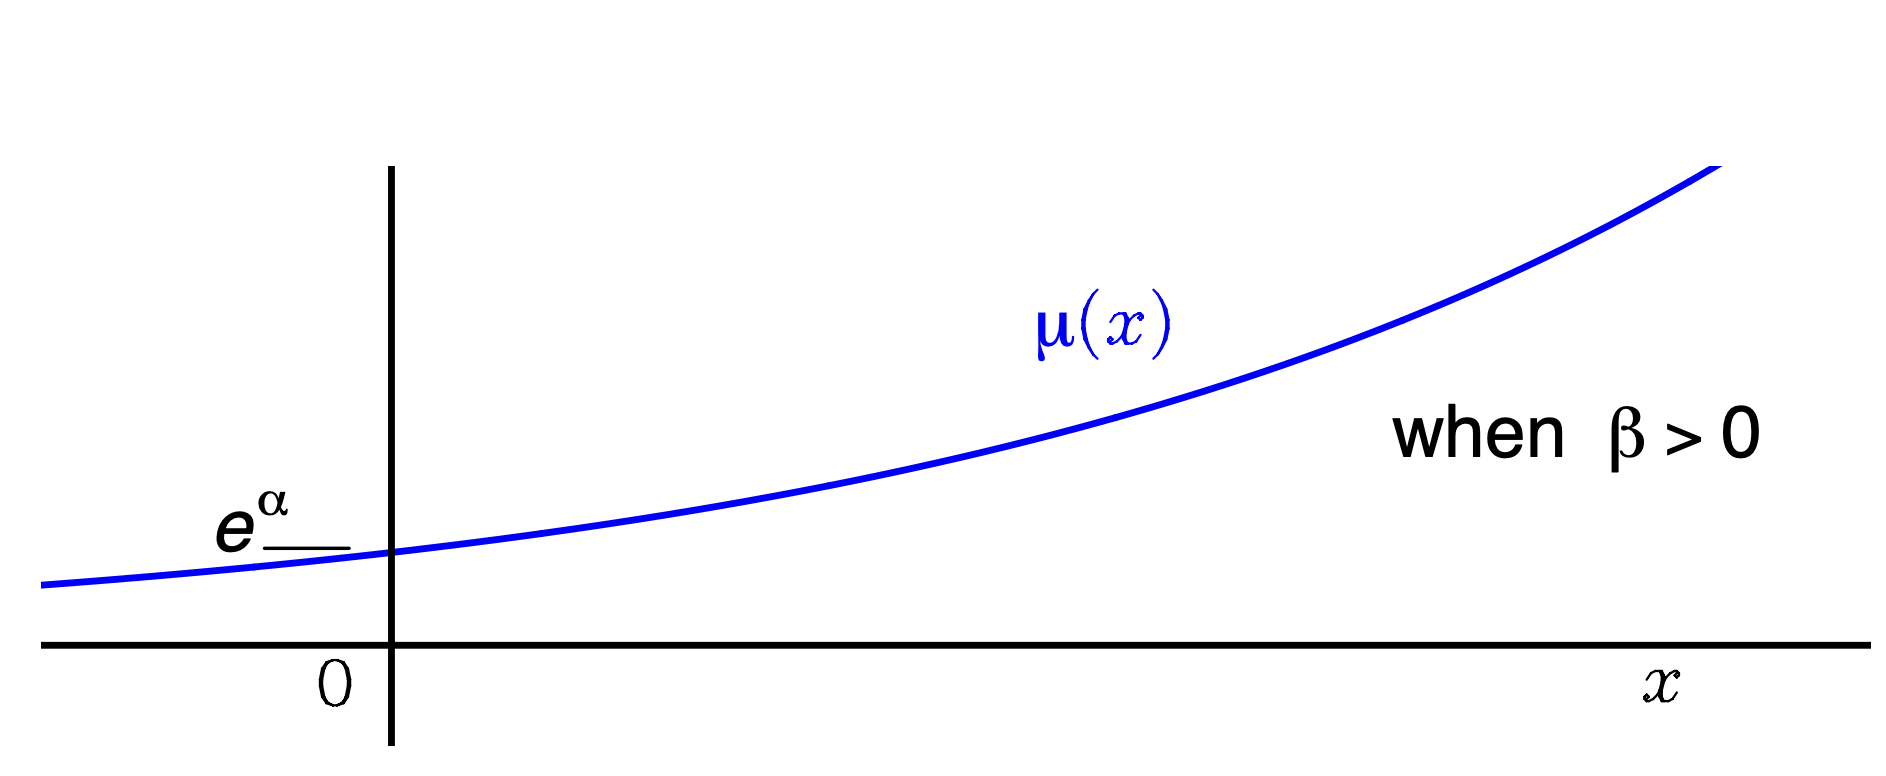
\includegraphics[scale=0.18]{logl.png}
        \caption{$\mu(x)=e^\alpha (e^\beta)^x$}
        \label{}
    \end{figure}\end{center}
\end{example}

\subsection{Rate Models}
$E\left(Y_i\right)=\mu_i$ is sometimes expected to be proportional to another observed variable $t_i>0$ :
$$
\mu_i=\lambda_i t_i
$$
e.g.
$$
\begin{aligned}
Y_i & =\text { cases of rare disease in nation } i \\
t_i & =\text { national population (known) } \\
\lambda_i & =\text { disease \textbf{rate} (unknown) }
\end{aligned}
$$
($t$ could alternatively be a temporal or spatial extent)\\
\textbf{Canonical link:}
$$
\begin{aligned}
\ln \mu_i & =\ln \lambda_i+\ln t_i \\
& =\alpha+\beta_1 x_{i 1}+\cdots+\beta_p x_{i p}+\ln t_i
\end{aligned}
$$
where $\lambda_i$ works as linear predictor, $\ln \lambda_i=\alpha+\beta_1 x_{i 1}+\cdots+\beta_p x_{i p}$\\
Note: $\ln t_i$ has no coefficient. We call $\ln t_i$ an \textbf{offset}.


\subsubsection*{For $2\times 2$ Tables}
\begin{table}[htbp]
    \centering
    \begin{tabular}{rcccc}
        \multicolumn{1}{r}{}&\multicolumn{2}{c}{$x_2=1$}&\multicolumn{2}{c}{$x_2=0$}\\
        \cline{2-5}
        \multicolumn{1}{r|}{$x=1$}&\multicolumn{2}{c|}{$Y_{11}$}&\multicolumn{2}{c|}{$Y_{12}$}\\
        \cline{2-5}
        \multicolumn{1}{r|}{$x=0$}&\multicolumn{2}{c|}{$Y_{21}$}&\multicolumn{2}{c|}{$Y_{22}$}\\
        \cline{2-5}
        \multicolumn{1}{c}{}&&&&
    \end{tabular}\\
    $\left\{Y_{i j}\right\} \sim \text { indep. Poisson }\left(\left\{\mu_{i j}\right\}\right)$
\end{table}
The full loglinear regression model can be parameterized as
$$
\ln \mu_{i j}=\alpha+\beta_1 x_1+\beta_2 x_2+\beta_3 x_1 x_2
$$
(Can solve for $\alpha, \beta_1, \beta_2, \beta_3$ in terms of the $\mu_{i j}$.)

Recall relation to multinomial:
$$
\begin{gathered}
\left\{Y_{i j}\right\} \mid \sum_{i j} Y_{i j}=n \sim \operatorname{multinomial}\left(n,\left\{\pi_{i j}\right\}\right) \\
\pi_{i j}=\frac{\mu_{i j}}{\mu_{11}+\mu_{12}+\mu_{21}+\mu_{22}}
\end{gathered}
$$
Recall odds ratio:
$$
\theta=\frac{\pi_{11} \pi_{22}}{\pi_{12} \pi_{21}}=\frac{\mu_{11} \mu_{22}}{\mu_{12} \mu_{21}}
$$
Can show $\theta=1$ (i.e., no association) is equivalent to $\beta_3=0$ (i.e., no interaction term):
$$
\ln \mu_{i j}=\alpha+\beta_1 x_1+\beta_2 x_2
$$


\section{Coefficient and Model Inferences}
\subsection*{Matrix Forms}
We can write the \textbf{linear predictor} of GLM
$$\eta_i = \alpha+\beta_1 x_{i1}+\cdots +\beta_p x_{ip},\quad i=1,...,N$$
in vector form: $$\boldsymbol{\eta}=\mathbf{X}\boldsymbol{\beta}$$
where $\boldsymbol{\eta}=\left[\eta_1,\cdots,\eta_N\right]^T$, $\boldsymbol{\beta}=\left[\alpha,\beta_1,\cdots, \beta_p\right]^T$, and the model matrix $\mathbf{X}$ has $i^\textnormal{th}$ row $[1,x_{i1},\cdots,x_{ip}]$.

Let the MLE of $\boldsymbol{\beta}$ be $$\hat{\boldsymbol{\beta}}=\left[\hat{\alpha},\hat{\beta}_1,\cdots,\hat{\beta}_p \right]^T$$

\subsection{Wald Inference}
\subsubsection{(Fisher) Information Matrix}
\begin{definition}[(Fisher) Information Matrix]
    \normalfont
    The (Fisher) information matrix for $\boldsymbol{\beta}\in \mathbb{R}^{p+1}$ is a $(p+1)\times(p+1)$ matrix $$\boldsymbol{\mathcal{J}}$$ with element $(h,j)$ being $$\mathbb{E}\left(-\frac{\partial^2 L(\boldsymbol{\beta})}{\partial \beta_h \partial \beta_j}\right)$$
\end{definition}
For a GLM, the information matrix becomes $$\boldsymbol{\mathcal{J}}=\mathbf{X}^T \mathbf{W} \mathbf{X}$$
where $\mathbf{W}=\textnormal{diag}\left(w_1,\cdots,w_N\right)$ with $$w_i=\left(\frac{\partial \mu_i}{\partial \eta_i}\right)^2\cdot \frac{1}{\textnormal{var}(Y_i)}$$
Recall $\mu_i=\mathbb{E}(Y_i)$.

\begin{example}[ Logistic Regression]
    $$
    \begin{gathered}
    \mu_i=E\left(Y_i\right)=n_i \pi_i \quad \operatorname{var}\left(Y_i\right)=n_i \pi_i\left(1-\pi_i\right) \\
    \eta_i=\operatorname{logit}\left(\pi_i\right)=\ln \pi_i-\ln \left(1-\pi_i\right)
    \end{gathered}
    $$
    Then
    $$
    \begin{aligned}
    \frac{\partial \mu_i}{\partial \eta_i} & =\frac{\partial \mu_i}{\partial \pi_i} \cdot \frac{\partial \pi_i}{\partial \eta_i}=n_i \cdot\left(\frac{\partial \eta_i}{\partial \pi_i}\right)^{-1} \\
    & =n_i\left(\frac{1}{\pi_i}+\frac{1}{1-\pi_i}\right)^{-1}=n_i \pi_i\left(1-\pi_i\right)
    \end{aligned}
    $$
    Thus
    $$
    w_i=\left(n_i \pi_i\left(1-\pi_i\right)\right)^2 \cdot \frac{1}{n_i \pi_i\left(1-\pi_i\right)}=n_i \pi_i\left(1-\pi_i\right)
    $$
\end{example}

\subsubsection{Wald Inference}
Under regularity conditions, as $N \rightarrow \infty$, the distribution of $\hat{\boldsymbol{\beta}}$ is approximately multivariate normal with mean vector $\boldsymbol{\beta}$ and covariance matrix $\boldsymbol{\mathcal{J}}^{-1}$ (a proposition in MLE part):
$$
\hat{\boldsymbol{\beta}}\quad \dot{\sim}\quad N\left(\boldsymbol{\beta}, \boldsymbol{\mathcal{J}}^{-1}\right)
$$
So the asymptotic covariance of $\hat{\boldsymbol{\beta}}$ is
$$
\boldsymbol{\mathcal{J}}^{-1}=\left(\boldsymbol{X}^T \boldsymbol{W} \boldsymbol{X}\right)^{-1}
$$
which is estimated as
$$
\widehat{\operatorname{cov}}(\hat{\boldsymbol{\beta}})=\left(\boldsymbol{X}^T \hat{\boldsymbol{W}} \boldsymbol{X}\right)^{-1}
$$
where $\hat{\boldsymbol{W}}$ is $\boldsymbol{W}$ estimated using $\hat{\boldsymbol{\beta}}$ for $\boldsymbol{\beta}$.

In particular, the element $\hat{\beta}_j$ of $\hat{\boldsymbol{\beta}}$ is asymptotically normal with asymptotic variance
$$
\widehat{\operatorname{var}}\left(\hat{\beta}_j\right)=(j+1) \text { st diagonal element of } \widehat{\operatorname{cov}}(\hat{\boldsymbol{\beta}})
$$
The Wald $z$ statistic for testing $H_0: \beta_j=\beta_{j 0}$ is
$$
z_W=\frac{\hat{\beta}_j-\beta_{j 0}}{S E\left(\hat{\beta}_j\right)}\quad \underset{\mathrm{H}_0}{\dot{\sim}}\quad N(0,1)
$$
where $S E\left(\hat{\beta}_j\right)=\sqrt{\widehat{\operatorname{var}}\left(\hat{\beta}_j\right)}$.

Also Wald Cls:
$$
\hat{\beta}_j \pm z_{\alpha / 2} \cdot S E\left(\hat{\beta}_j\right)
$$





\subsection{Deviance  and Likelihood-Ratio Test}
\subsubsection{ Deviance and Goodness of Fit}
Then it can be shown that $\boldsymbol{\mu}=\boldsymbol{y}$ maximizes $L$.
It follows that
$$
L(\boldsymbol{y} ; \boldsymbol{y}) \geq L(\hat{\boldsymbol{\mu}} ; \boldsymbol{y})
$$
where $\hat{\boldsymbol{\mu}}$ is the MLE of $\boldsymbol{\mu}$ (when it exists) for the GLM.
The unrestricted case, in which each observation has its own mean, is called the \textbf{saturated model}.

\begin{definition}[Deviance]
    \normalfont
    The \textbf{deviance} of the GLM is
    $$
    D(\boldsymbol{y} ; \hat{\boldsymbol{\mu}})=-2(L(\hat{\boldsymbol{\mu}} ; \boldsymbol{y})-L(\boldsymbol{y} ; \boldsymbol{y}))
    $$
    Note: $D(\boldsymbol{y} ; \hat{\boldsymbol{\mu}})$ is the \underline{likelihood-ratio test (LRT) chi-squared statistic $G^2$} for
    \begin{enumerate}[-]
        \item $H_0$ : the GLM is correct
        \item $H_a$ : the GLM is incorrect
        (but the saturated model is correct)
    \end{enumerate}
\end{definition}
The deviance is associated with \underline{degrees of freedom}
$$
\begin{aligned}
\mathrm{df} & =\# \text { means in sat. model }-\# \text { params. in GLM } \\
& =N-(p+1) \quad \text { (usually) }
\end{aligned}
$$

For a $2 \times 2$ table, for the independent binomial model under homogeneity ($\pi_1 = \pi_2$), $D(\boldsymbol{y} ; \hat{\boldsymbol{\mu}})$ is $G^2$ for testing homogeneity. The notion for model $M$'s deviance is $G^2(M)$, that is a model $M$'s deviance is
\begin{equation}
    \begin{aligned}
        G^2(M)=D(\boldsymbol{y} ; \hat{\boldsymbol{\mu}})=-2(L(\hat{\boldsymbol{\mu}} ; \boldsymbol{y})-L(\boldsymbol{y} ; \boldsymbol{y}))
    \end{aligned}
    \nonumber
\end{equation}

\subsubsection{Goodness of Fit Test / Likelihood-Ratio Test}
Under certain asymptotic conditions,
$$
D(\boldsymbol{y} ; \hat{\boldsymbol{\mu}})\quad \underset{\mathrm{H}_0}{\dot{\sim}} \quad \chi_{\mathrm{df}}^2
$$
and tends larger under $H_\alpha$.

So reject correctness of the GLM if
$$
D(\boldsymbol{y} ; \hat{\boldsymbol{\mu}})>\chi_{\mathrm{df}}^2(\alpha)
$$
(or use a $P$-value).

\textbf{Warning:} Chi-squared approximation can be poor. The chi-squared approximation (under $H_0$ ) is adequate if all
$$
\mu_i=n_i \pi_i \quad \text { and } \quad n_i-\mu_i=n_i\left(1-\pi_i\right)
$$
are sufficiently large.

The chi-squared approximation is never valid for binary responses ($n_i=1$, i.e. ungrouped data). Indeed, in that case, the deviance is completely useless for model checking.

\begin{example}[ Poisson Case]
    For a (Poisson) loglinear model, $L(\boldsymbol{\mu};\boldsymbol{y})=\sum_{i} \ln \left(\frac{\mu_i^{y_i}}{y_i !} e^{-\mu_i}\right)$, we can show
    \begin{equation}
        \begin{aligned}
            D(\boldsymbol{y} ; \hat{\boldsymbol{\mu}})&=2\sum_i \left(y_i\ln\frac{y_i}{\hat{\mu}_i}-y_i+\hat{\mu}_i\right)\\
            &=2\sum_i y_i\ln\frac{y_i}{\hat{\mu}_i}
        \end{aligned}
        \nonumber
    \end{equation}
    \textbf{Remark:}
    \begin{enumerate}[$\bullet$]
        \item The chi-squared approximation (under $H_0$) is adequate if all $\mu_i$ are sufficiently large.
        \item These formulas also apply to loglinear rate models (with rate variable $t_i$), for which $\mu_i=\lambda_i t_i$, $\hat{\mu}_i=\hat{\lambda}_i t_i$, where $\hat{\lambda}_i$ is the MLE of rate $\lambda_i$.
    \end{enumerate}
\end{example}
\begin{example}[ Binomial Case]
    $Y_i\sim \textnormal{binomial}(n_i,\pi_i)$, $L(\boldsymbol{\mu};\boldsymbol{y})=\sum_{i} \ln \left(\frac{\mu_i}{n_i}\right)^{y_i}\left(1-\frac{\mu_i}{n_i}\right)^{n_i-y_i}$
    \begin{equation}
        \begin{aligned}
            D(\boldsymbol{y} ; \hat{\boldsymbol{\mu}})=2\sum_i y_i\ln\frac{y_i}{\hat{\mu}_i}+2\sum_i(n_i-y_i)\ln \frac{n_i-y_i}{n_i-\hat{\mu}_i}
        \end{aligned}
        \nonumber
    \end{equation}
    where $\hat{\mu}_i=n_i\hat{\pi}_i$. (Convention: $0\ln 0=0$)\\
    \textbf{Remark:} If the data is $N\times 2$, this deviance is the same as the deviance for the Poisson model with $2N$ observations.
\end{example}


\subsection{Nested Model Comparison}
“Nested” means that one model is a subset of another.
\begin{definition}[Nested Model]\normalfont
    Model $M_0$ is \textbf{nested} in Model $M_1$ if the parameters in Model $M_0$ are a subset of the parameters in Model $M_1$. E.g.
    \begin{equation}
        \begin{aligned}
            M_0:\quad g(\mu_i)&=\alpha+\beta_1 x_{i1}+\cdots +\beta_{p_0} x_{ip_0}\\
            M_1:\quad g(\mu_i)&=\alpha+\beta_1 x_{i1}+\cdots +\beta_{p_1} x_{ip_1}
        \end{aligned}
        \nonumber
    \end{equation}
    where $p_0<p_1$. That is, $\boldsymbol{\mu}$ is more restricted under $M_0$ than under $M_1$.
\end{definition}
Let $\hat{\boldsymbol{\mu}}_0$ be the MLE under $M_0$ and $\hat{\boldsymbol{\mu}}_1$ be the MLE under $M_1$.

For testing
$$
H_0: M_0 \text { true } \quad H_a: M_1 \text { true, but not } M_0
$$
the LRT chi-squared statistic is
$$
\begin{aligned}
&-2\left(L\left(\hat{\boldsymbol{\mu}}_0 ; \boldsymbol{y}\right)-\right. \left.L\left(\hat{\boldsymbol{\mu}}_1 ; \boldsymbol{y}\right)\right)\\
= & -2\left(L\left(\hat{\boldsymbol{\mu}}_0 ; \boldsymbol{y}\right)-L(\boldsymbol{y} ; \boldsymbol{y})\right)  -\left[-2\left(L\left(\hat{\boldsymbol{\mu}}_1 ; \boldsymbol{y}\right)-L(\boldsymbol{y} ; \boldsymbol{y})\right)\right] \\
= & D\left(\boldsymbol{y} ; \hat{\boldsymbol{\mu}}_0\right)-D\left(\boldsymbol{y} ; \hat{\boldsymbol{\mu}}_1\right)
\end{aligned}
$$
which is always non-negative.

If the chi-squared approximation is adequate, reject $H_0$ if
$$
D\left(\boldsymbol{y} ; \hat{\boldsymbol{\mu}}_0\right)-D\left(\boldsymbol{y} ; \hat{\boldsymbol{\mu}}_1\right)>\chi_{\mathrm{df}}^2(\alpha)
$$
where
$$
\begin{aligned}
\mathrm{df}= & \text { effective \# params. in } M_1 -\text { effective \# params. in } M_0
\end{aligned}
$$
\textbf{Remark:} The chi-squared approximation is often adequate here even when it isn't adequate for the saturated model (provided $M_1$ is not too close to saturated).

\textbf{Notation:} For comparing null model $M_0$ to larger model $M_1$, denote the LRT chi-squared statistic as $$G^2(M_0\mid M_1)=D\left(\boldsymbol{y} ; \hat{\boldsymbol{\mu}}_0\right)-D\left(\boldsymbol{y} ; \hat{\boldsymbol{\mu}}_1\right)=-2\left(L\left(\hat{\boldsymbol{\mu}}_0 ; \boldsymbol{y}\right)-\right. \left.L\left(\hat{\boldsymbol{\mu}}_1 ; \boldsymbol{y}\right)\right)$$

\begin{definition}[Profile Likelihood CIs]
    \normalfont
    Say we want a $\mathrm{Cl}$ for a parameter $\beta$ in a model $M_1$.\\
    Let
    $$
    M_0\left(\beta_0\right)=\text { same model, except } \beta \text { is fixed at } \beta_0
    $$
    Then the LRT tests
    $$
    H_0: \beta=\beta_0 \quad H_a: \beta \neq \beta_0
    $$
    and produces a $P$-value (from chi-squared approximation).\\
    Then
    $$
    \left\{\beta_0: P \text {-value }>\alpha\right\}
    $$
    is an approx. $(1-\alpha) 100 \%$ confidence set (usually a $\mathrm{Cl}$ ) for $\beta$.\\
    This interval (based on the test inversion idea) is a \textbf{profile likelihood CI}.
\end{definition}

\subsection{Residuals}
As in linear regression, residuals provide a way to examine lack of fit: patterns of departure from the model, and "outliers."
Recall $\hat{\mu}_i=\mathrm{MLE} \text { of } E\left(Y_i\right)$. The raw residuals $y_i-\hat{\mu}_i$
have unequal variances, making it difficult to use them to examine lack of fit.

\begin{definition}[Pearson Residuals]
    \normalfont
    $$
    e_i=\frac{y_i-\hat{\mu}_i}{\sqrt{\nu\left(\hat{\mu}_i\right)}}
    $$
    where $\nu(\mu)=\operatorname{var}(Y)$.\\
    When $\operatorname{var}(Y)=\mu$, eg: Poisson
    $$
    e_i=\frac{y_i-\hat{\mu}_i}{\sqrt{\hat{\mu}_i}}
    $$
\end{definition}

\begin{definition}[Deviance Residuals]
    \normalfont
    The deviance can be written in terms of the sum of contributions from each observation $D(\boldsymbol{y} ; \hat{\boldsymbol{\mu}})=\sum_{i=1}^N d_i
    $, where $d_i=-2\left(L\left(\hat{\mu}_i ; y_i\right)-L\left(y_i ; y_i\right)\right)$ is non-negative.\\
    The $i^\textnormal{th}$ \textbf{deviance residual} is $$\operatorname{sign}\left(y_i-\hat{\mu}_i\right) \cdot \sqrt{d_i}
    $$
\end{definition}
\textbf{Problem:} Neither Pearson nor deviance residuals are truly standardized. Their variances tend to be less than 1, and often unequal. Need a type of residual that (approximately) fixes these problems.

\begin{definition}[Standardized Residuals]
    \normalfont
    $$
    r_i=\frac{y_i-\hat{\mu}_i}{\sqrt{\nu\left(\hat{\mu}_i\right)\left(1-\hat{h}_i\right)}}=\frac{e_i}{\sqrt{1-\hat{h}_i}}
    $$
    where $\hat{h}_i$ is the $i^\textnormal{th}$ \textbf{leverage}.

    The \textbf{leverages} are the diagonal elements of the (estimated) \textbf{hat matrix}
    $$
    \hat{\boldsymbol{H}}_{a t}=\hat{\boldsymbol{W}}^{1 / 2} \boldsymbol{X}\left(\boldsymbol{X}^T \hat{\boldsymbol{W}} \boldsymbol{X}\right)^{-1} \boldsymbol{X}^T \hat{\boldsymbol{W}}^{1 / 2}
    $$
    where $\hat{\boldsymbol{W}}^{1 / 2}$ is the diagonal matrix of square roots of the diagonal elements of $\hat{\boldsymbol{W}}$.
\end{definition}
\textbf{Remark:} A leverage measures “potential influence” of its observation — how sensitively the fit depends on it.

\subsection{Overdispersion}
Recall: In our GLMs, $\operatorname{var}(Y)$ is a function of $\mu=E(Y)$.
\begin{definition}[Overdispersion]
    \normalfont
    \textbf{Overdispersion} is when $\operatorname{var}(Y)$ for the data appears larger than the fitted $\mu$ predicts.\\
    This is common in Poisson regression, and sometimes in binomial.\\
    (\textbf{Underdispersion}, in which $\operatorname{var}(Y)$ is smaller than predicted, is rare.)\\
    Overdispersion is a type of lack of fit, and may cause a goodness of fit test to reject.
\end{definition}
Under the GLM, let $\nu^*(\mu)=\operatorname{var}(Y)$, the \textbf{overdispersion} is when
\begin{equation}
    \begin{aligned}
        \textnormal{actual var}(Y)>\nu^*(\mu)
    \end{aligned}
    \nonumber
\end{equation}

\subsubsection*{Possible \underline{causes} of overdispersion:}
\begin{enumerate}
    \item heterogeneity among observations (variations in $\mu$ not captured by the model)
    \item lurking variables (unused predictors, possibly unknown)
    \item correlations among observations (e.g. clustering)
\end{enumerate}

\subsubsection*{One remedy: quasi-likelihood}
Use a \textbf{quasi-likelihood} having an additional \textbf{dispersion parameter} $\phi>0$ that scales the variance:
\begin{equation}
    \begin{aligned}
        \nu_\phi(\mu)=\phi\nu^*(\mu)
    \end{aligned}
    \nonumber
\end{equation}
E.g., for Poisson, $\nu_\phi(\mu)=\phi\mu$. Then $\phi > 1$ represents overdispersion.

Under quasi-likelihood, the estimate of $\boldsymbol{\beta}$ (and thus $\boldsymbol{\mu}$ ) remains unchanged: $\hat{\boldsymbol{\beta}}$ is still the MLE from the original model.

Usually $\phi$ is estimated as
$$
\hat{\phi}=\frac{X^2}{N-p^{\prime}},\quad\textnormal{ where }
X^2=\sum_i \frac{\left(y_i-\hat{\mu}_i\right)^2}{\nu^*\left(\hat{\mu}_i\right)}
$$
and $p^{\prime}$ is the effective number of parameters in $\boldsymbol{\beta}$ (usually $p+1$).

We can use the $\hat{\phi}$ to scale the GLM asymptotic covariance of $\hat{\boldsymbol{\beta}}$. In particular, the new (adjusted) $S E\left(\hat{\beta}_j\right)$ is just the GLM version multiplied by $\sqrt{\hat{\phi}}$. Then use the new standard errors for Wald-type inference.

\textbf{Remark:} Similar adjustments apply to likelihood-type and score-type inferences.

\chapter{Binary-Response Regression except Logistic Regression}
\section{Probit Model}
\subsection{Probit Link}
The probit link is $$g(\pi)=\Phi^{-1}(\pi)$$ where $\Phi = \textnormal{ c.d.f. of }N(0,1)$. Using the probit link is \textbf{probit regression}.
\subsection{Motivation: Latent Response}

Suppose there is just a single explanatory variable $x$, and it is quantitative.

Consider ordinary simple linear regression with a response $Y^*$ :
$$
Y^* \sim N(\alpha+\beta x, 1)
$$
assuming variance $\sigma^2$ is equal to $1$.

Suppose $Y^*$ is latent (unobserved), but we observe
$$
Y=\left\{\begin{array}{lll}
1 & \text { if } & Y^*>0 \\
0 & \text { if } & Y^* \leq 0
\end{array}\right.
$$
Then
$$
\begin{aligned}
\pi(x) & =\mathrm{P}(Y=1 \mid x) \\
& =\mathrm{P}\left(Y^*>0 \mid x\right) \\
& =\mathrm{P}\left(Y^*-\alpha-\beta x>-\alpha-\beta x \mid x\right) \\
& =\mathrm{P}(Z>-\alpha-\beta x) \quad(Z \text { standard normal) } \\
& =\mathrm{P}(Z<\alpha+\beta x) \quad \text { (symmetry) } \\
& =\Phi(\alpha+\beta x)
\end{aligned}
$$
So $Y$ satisfies a probit regression.

\subsection{Properties and Interpretation}
Again consider one quantitative $x$ variable:
$$
\pi(x)=\Phi(\alpha+\beta x)
$$
Then
$$
\frac{d \pi(x)}{d x}=\beta \phi(\alpha+\beta x)
$$
where $\phi=\text { density of } N(0,1)$.\\
If $\beta \neq 0$, slope is steepest at
$$
x=-\frac{\alpha}{\beta} \quad(\text {where } \alpha+\beta x=0)
$$
Relation to latent response $Y^*$ :
\begin{center}
    a unit increase in $x$ implies an increase of $\beta$ in $E\left(Y^*\right)$
(which is a decrease if $\beta<0$)
\end{center}
This assumes $\operatorname{var}\left(Y^*\right)=1$. (Otherwise, the increase is in standard deviation units - later.)

Sign of $\beta$ indicates direction of $X-Y^*$ relationship.

\subsection{Model Fitting and Checking}
Usually fit by maximum likelihood to get $\hat{\boldsymbol{\beta}}$.

Can use deviance (or Pearson $X^2$) to check fit.

Residuals and influence measures are also available. Fitted values are defined as usual.

Remark: Fisher scoring and Newton-Raphson algorithms are different for probit regression, and can cause software to report different standard errors.

\subsection{Inference}
Assume the general (binomial) form for the data:
$$
\begin{gathered}
Y_i \sim \text { indep. binomial }\left(n_i, \pi\left(\boldsymbol{x}_i\right)\right) \\
\Phi^{-1}\left(\pi\left(\boldsymbol{x}_i\right)\right)=\eta_i=\boldsymbol{x}_i^T \boldsymbol{\beta} \\
\boldsymbol{x}_i^T=i^\textnormal{th} \text { row of } \boldsymbol{X} \quad \boldsymbol{\eta}=\boldsymbol{X} \boldsymbol{\beta}
\end{gathered}
$$
The estimated asymptotic covariance (obtained by inverting estimated information):
$$
\widehat{\operatorname{cov}}(\hat{\boldsymbol{\beta}})=\left(\boldsymbol{X}^T \hat{\boldsymbol{W}} \boldsymbol{X}\right)^{-1}
$$
with
$$
\hat{\boldsymbol{W}}=\operatorname{diag}\left(n_i \frac{\left(\phi\left(\hat{\eta}_i\right)\right)^2}{\Phi\left(\hat{\eta}_i\right)\left(1-\Phi\left(\hat{\eta}_i\right)\right)}\right)
$$
where
$$
\hat{\eta}_i=\boldsymbol{x}_i^T \hat{\boldsymbol{\beta}}
$$
This can be used for Wald inference. Likelihood-ratio and score inference are also available.

\subsection{Variance $\sigma^2\neq 1$}
Suppose we allow the latent variable to have an unknown variance $\sigma^2$, so that
$$
Y^* \sim N\left(\tilde{\alpha}+\tilde{\beta} x, \sigma^2\right)
$$
where $\sigma^2>0$ is arbitrary.

As before, observe
$$
Y=\left\{\begin{array}{lll}
1 & \text { if } & Y^*>0 \\
0 & \text { if } & Y^* \leq 0
\end{array}\right.
$$
It turns out that $\tilde{\alpha}, \tilde{\beta}$, and $\sigma^2$ are not identifiable, so can't be estimated ...
$$
\begin{aligned}
\pi(x) & =\mathrm{P}(Y=1 \mid x)=\mathrm{P}\left(Y^*>0 \mid x\right) \\
& =\mathrm{P}\left(\frac{Y^*-\tilde{\alpha}-\tilde{\beta} x}{\sigma}>\frac{0-\tilde{\alpha}-\tilde{\beta} x}{\sigma} \mid x\right) \\
& =\mathrm{P}(Z>-\tilde{\alpha} / \sigma-\tilde{\beta} x / \sigma) \quad(Z \text { standard normal) } \\
& =\mathrm{P}(Z<\tilde{\alpha} / \sigma+\tilde{\beta} x / \sigma) \quad \text { (symmetry) } \\
& =\Phi(\underbrace{\tilde{\alpha} / \sigma}_\alpha+\underbrace{(\tilde{\beta} / \sigma)}_\beta x)
\end{aligned}
$$
Probit regression estimates $\alpha$ and $\beta$, not $\tilde{\alpha}$ and $\tilde{\beta}$.

Thus, when $\sigma^2 \neq 1, \alpha$ and $\beta$ must be interpreted in standard deviation units.

Eg: Increasing $x$ by 1
\begin{center}
    increases $E\left(Y^*\right)$ by $\tilde{\beta}=\sigma \beta$
\end{center}
i.e., by $\beta$ standard deviations.

Again, $\tilde{\alpha}, \tilde{\beta}$, and $\sigma^2$ are not identified, so can't be estimated.

\subsection{Symmetry Property}
Logit and probit links have the symmetry property
$$g(\pi) = -g(1 - \pi)$$
This means both tails exhibit the same asymptotic behavior.

An implication: If
$$
Y_i \sim \operatorname{binomial}\left(n_i, \cdot\right)
$$
follows a logistic (or probit) model with parameter $\boldsymbol{\beta}$, then
$$
n_i-Y_i
$$
follows a logistic (or probit) model with parameter $-\boldsymbol{\beta}$.
This property is convenient, since the model is equivalent no matter which type of outcome is designated as the "success" and which the "failure."
However, sometimes an asymmetric model fits the data better.

\section{Complementary Log-Log Model}
The complementary log-log link is
$$
g(\pi)=\ln (-\ln (1-\pi))
$$
The corresponding "response curve":
$$
\pi(\eta)=g^{-1}(\eta)=1-e^{-e^\eta}
$$
Property: When $\eta=\alpha+\beta x$,
$$(1-\pi(x_2))=(1-\pi(x_1))^{e^{\beta(x_2-x_1)}}$$
Remarks:
\begin{enumerate}[$\bullet$]
    \item This link does not have the symmetry property - the model does depend on which type of outcome is the "success."
    \item There is also a log-log link, which is obtained by interchanging the roles of "success" and "failure."
\end{enumerate}

\chapter{Logistic Regression}
\section{Parameter Interpretation of (Simple) Logistic Regression}
Suppose we observe $0 / 1$ (Bernoulli) response $Y$ and quantitative explanatory variable $X$.
Let
$$
\pi(x)=\mathrm{P}(Y=1 \mid X=x) \quad \in(0,1) \text { for all } x
$$
The (simple) logistic regression of $Y$ on $X$ uses
$$
\pi(x)=\frac{e^{\alpha+\beta x}}{1+e^{\alpha+\beta x}}
$$
i.e.
$$
\operatorname{logit}(\pi(x))=\ln \left(\frac{\pi(x)}{1-\pi(x)}\right)=\alpha+\beta x
$$
\subsection{Interpretation $\beta$}
Note: $"\text {odds of } Y=1"=\frac{\pi(x)}{1-\pi(x)}=e^{\alpha+\beta x}$\\
Odds ratio for $Y=1$ at $x+1$ versus at $x$: $\frac{e^{\alpha+\beta(x+1)}}{e^{\alpha+\beta x}}=e^\beta$, which doesn't depend on $x$.\\
So $\beta$ is the \textbf{log-odds ratio for the effect of increasing $X$ by one unit}.

We can also show $$\frac{d}{d x} \pi(x)=\beta \pi(x)(1-\pi(x))$$
The \textbf{median effective level} is the $x=-\frac{\alpha}{\beta}$ (if $\beta\neq 0$) at which $\pi(x) = \frac{1}{2}$ and the $\pi(x)$ is the steepest.

$\beta$ determines nature of $X-Y$ relationship:
\begin{enumerate}[-]
    \item $\beta>0$ : increasing $X$ increases prob. $Y=1$
    \item $\beta=0$ : no relationship
    \item $\beta<0$ : increasing $X$ decreases prob. $Y=1$
    Can show
\end{enumerate}

\subsection{Interpretation $\alpha$}
Interpreting $\alpha$ can be more difficult: it's the log-odds when $x = 0$.

If a mean-centered version of $X$ is used ($\mathbb{E}X=0$), $\alpha$ is the log-odds at the sample mean of the original $X$.

\section{Inference}
Assume independently-sampled data pairs $(x_i,y_i), i=1,...,N$. Let $\hat{\alpha},\hat{\beta}$ be the MLEs.

\subsection{Testing}
We still use three testing methods: 1. Wald; 2. Likelihood ratio; 3. Score (“Rao”).

Eg: Wald $z$-statistic for
$$
H_0: \beta=0 \quad H_a: \beta \neq 0
$$
is
$$
\frac{\hat{\beta}}{S E(\hat{\beta})}\quad \underset{H_0}{\dot{\sim}}\quad N(0,1)
$$
where the square of $S E$ comes from the estimated asymptotic covariance matrix (estimated inverse information matrix).

Similarly, we can form a Wald $\mathrm{Cl}$ for $\beta$: $(L,U)$.

Then, odds ratio $e^\beta$ for increasing $x$ by one unit is estimated by $e^{\hat{\beta}}$ and has CI $(e^L,e^U)$.

\subsection{Estimation}
Estimated logistic curve:
$$
\hat{\pi}(x)=\operatorname{logit}^{-1}(\hat{\alpha}+\hat{\beta} x)
$$
with estimated slope
$$
\hat{\beta} \hat{\pi}(x)(1-\hat{\pi}(x))
$$
So the estimated median effective level $(x$ such that $\hat{\pi}(x)=1 / 2)$ is $-\frac{\hat{\alpha}}{\hat{\beta}}$ if $\hat{\beta} \neq 0$.

For possible $X$ value $x_0$, we estimate $\pi(x_0)=P(Y=1\mid X=x_0)$ with $\hat{\pi}(x_0)$.

Note: $S E\left(\operatorname{logit} \hat{\pi}\left(x_0\right)\right)$ is the square root of
$$
\begin{aligned}
\widehat{\operatorname{var}}\left(\operatorname{logit} \hat{\pi}\left(x_0\right)\right) & =\widehat{\operatorname{var}}\left(\hat{\alpha}+\hat{\beta} x_0\right) \\
& =\widehat{\operatorname{var}}(\hat{\alpha})+x_0^2 \widehat{\operatorname{var}}(\hat{\beta})+2 x_0 \widehat{\operatorname{cov}}(\hat{\alpha}, \hat{\beta})
\end{aligned}
$$
where the estimated variances and covariance are from the estimated asymptotic covariance matrix.

The Wald Cl
$$
\operatorname{logit} \hat{\pi}\left(x_0\right) \pm z_{\alpha / 2} S E\left(\operatorname{logit} \hat{\pi}\left(x_0\right)\right)
$$
can be transformed (inverse logit) to a Wald $\mathrm{Cl}$ for $\pi\left(x_0\right)$.

\subsection{Testing Goodness of Fit; Remarks on Grouping}
Various strategies:
\begin{enumerate}[$\bullet$]
    \item Test an added higher-order term, e.g. test $\beta_2 = 0$ in the quadratic $$\alpha + \beta_1 x + \beta_2 x^2$$
    \item If there are \textbf{replicates} (repeated x values), use \textbf{grouped}
    (binomial) data to test using the deviance $D(\boldsymbol{y} ; \hat{\boldsymbol{\mu}})$\\
    Remarks on \underline{grouping}:
    \begin{enumerate}[1.]
        \item \underline{MLEs and likelihood-based inference for parameters remain the same}, since grouping doesn't change the kernel of the likelihood.
        \item The \underline{deviance changes}, since the saturated model for the grouped data is different.
        \item But \underline{deviance-based comparisons between nested sub-models do not change}, since the saturated model log-likelihood cancels out.
        \item A deviance-based goodness of fit test may be \underline{valid} for the grouped data, provided the values of $\mathbb{E}(Y_i)$ and $n_i - \mathbb{E}(Y_i)$ are \underline{not too small}.
        \item Note: “Fitted values” from R are still the probabilities $\hat{\pi}(x_i)$ (rather than estimated means $n_i\hat{\pi}(x_i)$).
    \end{enumerate}
\end{enumerate}

\section{Categorical Predictors}
Consider categorical $X$ with $I$ categories.

After grouping, we obtain an $I \times 2$ table:

\begin{center}
    \begin{tabular}{cc|c|c|}
        \multicolumn{2}{c}{ } & \multicolumn{1}{c}{ success } & \multicolumn{1}{c}{ failure } \\
        \cline { 3 - 4 } & $1$ & $Y_1$ & $n_1-Y_1$ \\
        $X$ category & $\vdots$ & $\vdots$ & $\vdots$ \\
        & $\vdots$ & $\vdots$ & $\vdots$ \\
        & $I$ & $Y_I$ & $n_I-Y_I$ \\
        \cline { 3 - 4 }
        \multicolumn{2}{c}{ } & \multicolumn{1}{c}{ } & \multicolumn{1}{c}{} \\
    \end{tabular}
\end{center}
Then $Y_i$ are i.i.d. variables following the binomial distribution.
$$
Y_i \sim \operatorname{binomial}\left(n_i, \pi_i\right) \quad i=1, \ldots, I
$$
\subsection{Interpretation of $\beta$}
Code $X$ using $I - 1$ indicator variables $\tilde{X}_i=[\tilde{x}_{i2},\tilde{x}_{i3},\cdots,\tilde{x}_{iI}]$ (No indicator variable for row $1$ to avoid redundancy.):
\begin{equation}
    \begin{aligned}
        \tilde{x}_{ij}=\left\{\begin{matrix}
            1,&\textnormal{ if }j=i\\
            0,&\textnormal{ otherwise}
        \end{matrix}\right.
    \end{aligned}
    \nonumber
\end{equation}
For logistic regression,
$$
\begin{aligned}
\operatorname{logit}\left(\pi_i\right) & =\alpha+\beta_2 \tilde{x}_{i 2}+\cdots+\beta_I \tilde{x}_{i I} \\
& =\alpha+\beta_i
\end{aligned}
$$
if we define $\beta_1 \equiv 0$. Then
$$
\begin{gathered}
\alpha=\operatorname{logit}\left(\pi_1\right) \\
\beta_i=\operatorname{logit}\left(\pi_i\right)-\operatorname{logit}\left(\pi_1\right)=\ln \left(\frac{\pi_i /\left(1-\pi_i\right)}{\pi_1 /\left(1-\pi_1\right)}\right) \\
=\text { log-odds ratio from category } i \text { to category } 1
\end{gathered}
$$
Similarly,
\begin{equation}
    \begin{aligned}
        \textnormal{$\beta_i-\beta_{i^{\prime}}=$ log-odds ratio from category $i$ to category $i^{\prime}$}
    \end{aligned}
    \nonumber
\end{equation}

\subsection{MLE Estimations}
MLEs of the $\pi_i$ s are
$$
\hat{\pi}_i=p_i=\frac{y_i}{n_i}
$$
and MLEs of $\alpha$ and $\beta_i$ are obtained from the empirical (or sample) logits
$$
\operatorname{logit}\left(\hat{\pi}_i\right)
$$
Letting $\beta_1 \equiv 0 \equiv \hat{\beta}_1$, we find
$$
\hat{\alpha}=\operatorname{logit}\left(\hat{\pi}_1\right) \quad \hat{\beta}_i=\operatorname{logit}\left(\hat{\pi}_i\right)-\hat{\alpha}
$$
For $i<i^{\prime}$,
$$
\hat{\beta}_i-\hat{\beta}_{i^{\prime}}\textnormal{ is the empirical log-odds ratio for the sub-table with only rows $i$ and $i^{\prime}$.}
$$
Note:
\begin{enumerate}[1.]
    \item If $y_i = 0$ or $y_i = n_i$, then $\operatorname{logit}\left(\hat{\pi}_i\right)$ does not exist, and thus neither does the MLE for the logistic regression.
    \item This model is saturated, so a deviance-based goodness of fit test is not available.
\end{enumerate}

\subsection{Testing}
Testing for any $X$ effect is testing
$$
\begin{aligned}
& H_0: \beta_2=\cdots=\beta_I=0 \quad\left(\equiv \beta_1\right) \\
& H_a: \text {not all } \beta_i \text { s equal (including $\beta_1$)}
\end{aligned}
$$
A LRT based on
$$
M_0: \operatorname{logit}\left(\pi_i\right)=\alpha \quad M_1: \operatorname{logit}\left(\pi_i\right)=\alpha+\beta_i
$$
uses $G^2\left(M_0 \mid M_1\right)$, which equals the $G^2$ statistic for testing independence/homogeneity in the $I \times 2$ table.

Alternative: The Pearson $X^2$ statistic.

\textbf{Remark:} When $X$ is ordinal, can sometimes improve power by assigning numerical scores $x_i^*$ to the $X$ levels and then using the linear logit model $$\textnormal{logit}(\pi_i)=\alpha+\beta x_i^*$$

\section{Multiple Logistic Regression}
Allow $p$ explanatory variables:
\begin{equation}
    \begin{aligned}
        \operatorname{logit}(\pi(\boldsymbol{x}))&=\alpha+\beta_1 x_1+\cdots+\beta_p x_p\\
        \pi(\boldsymbol{x})&=\frac{e^{\alpha+\beta_1 x_1+\cdots+\beta_p x_p}}{1+e^{\alpha+\beta_1 x_1+\cdots+\beta_p x_p}}
    \end{aligned}
    \nonumber
\end{equation}
$"\text{odds of } Y=1"=\frac{\pi(\boldsymbol{x})}{1-\pi(\boldsymbol{x})}=e^{\alpha+\beta_1 x_1+\cdots+\beta_p x_p}$.

Increasing just $x_j$ by 1 increases the logit by $\beta_j$, so
$$
e^{\beta_j}=\text { odds ratio at } x_j+1 \text { relative to } x_j
$$
(all other variables held fixed)

More generally, consider adding $\Delta x_j$ to $x_j, j=1, \ldots, p$. Using matrix notation let
$$
\mathbf{x}=\left(\begin{array}{c}
1 \\
x_1 \\
\vdots \\
x_p
\end{array}\right) \quad \boldsymbol{\delta}=\left(\begin{array}{c}
0 \\
\Delta x_1 \\
\vdots \\
\Delta x_p
\end{array}\right) \quad \boldsymbol{\beta}=\left(\begin{array}{c}
\alpha \\
\beta_1 \\
\vdots \\
\beta_p
\end{array}\right)
$$
\begin{enumerate}[$\bullet$]
    \item In this notation, $\operatorname{logit}(\pi(\mathbf{x}))=\mathbf{x}^T \boldsymbol{\beta}$
    \item Adding $\boldsymbol{\delta}$ to $\mathrm{x}$ adds $\boldsymbol{\delta}^T \boldsymbol{\beta}$ to the logit, so
    $$
    e^{\boldsymbol{\delta}^T \boldsymbol{\beta}}=\text { odds ratio at } \mathbf{x}+\boldsymbol{\delta} \text { relative to } \mathbf{x}
    $$
\end{enumerate}

\section{Matrix-Vector Formulation of Estimation}
$$
Y_i \sim \text { indep. binomial }\left(n_i, \pi\left(\boldsymbol{x}_i\right)\right)
$$
where $\boldsymbol{x}_i$ is the column vector of explanatory variable values for observation $i$, and (typically) a 1 for the intercept, and
$$
\operatorname{logit}\left(\pi\left(\boldsymbol{x}_i\right)\right)=\eta_i=\boldsymbol{x}_i^T \boldsymbol{\beta}
$$
Let
$$
\begin{aligned}
\boldsymbol{Y} & =\text { column vector with } i \text { th element } Y_i \\
\boldsymbol{X} & =\text { matrix with } \boldsymbol{x}_i^T \text { as } i \text { th row } \\
\boldsymbol{\eta} & =\text { column vector with } i \text { th element } \eta_i
\end{aligned}
$$

\subsubsection*{Log-Likelihood}
Note:$\boldsymbol{\eta}=\boldsymbol{X} \boldsymbol{\beta}$, $\pi\left(\boldsymbol{x}_i\right)=\frac{e^{\eta_i}}{1+e^{\eta_i}}$, and
\begin{equation}
    \begin{aligned}
        l(\boldsymbol{\beta})&=\prod_{i}\begin{pmatrix}
            n_i\\
            y_i
        \end{pmatrix} \pi\left(\boldsymbol{x}_i\right)^{y_i} (1-\pi\left(\boldsymbol{x}_i\right))^{n_i-y_i}\\
        L(\boldsymbol{\beta})&=\sum_{i}\left[ y_i\ln\pi\left(\boldsymbol{x}_i\right)+(n_i-y_i)\ln(1-\pi\left(\boldsymbol{x}_i\right))\right]\\
        &=\sum_{i}\left[ y_i(\eta_i-\ln\left(1+e^{\eta_i}\right))-(n_i-y_i)\ln\left(1+e^{\eta_i}\right)\right]\\
        &=\sum_{i}\left[y_i\eta_i-n_i\ln\left(1+e^{\eta_i}\right)\right]
    \end{aligned}
    \nonumber
\end{equation}
The log-likelihood (binomial response) is
$$
L(\boldsymbol{\beta})=\boldsymbol{y}^T \boldsymbol{X} \boldsymbol{\beta}-\sum_i n_i \ln \left(1+e^{\eta_i}\right)
$$
where $\boldsymbol{y}$ is the observed version of $\boldsymbol{Y}$.

\subsubsection*{Score Vector}
The score vector is
$$
\begin{aligned}
\boldsymbol{u}(\boldsymbol{\beta})=\nabla L(\boldsymbol{\beta}) & =\boldsymbol{X}^T \boldsymbol{y}-\sum_i n_i \boldsymbol{x}_i \pi\left(\boldsymbol{x}_i\right) \\
& =\boldsymbol{X}^T \boldsymbol{y}-\boldsymbol{X}^T \boldsymbol{\mu}
\end{aligned}
$$
where $\boldsymbol{\mu}=E(\boldsymbol{Y})$\\
This equals $\mathbf{0}$ at the MLE, giving the likelihood equations
$$
\boldsymbol{X}^T \boldsymbol{y}=\boldsymbol{X}^T \hat{\boldsymbol{\mu}}
$$
(Note: $\boldsymbol{y}-\hat{\boldsymbol{\mu}}$ is orthogonal to the columns of $\boldsymbol{X}$, just like in linear regression.)

\subsubsection*{Information Matrix and Covariance}
The second derivative matrix is
$$
\begin{aligned}
\nabla^2 L(\boldsymbol{\beta}) & =-\sum_i n_i \boldsymbol{x}_i \boldsymbol{x}_i^T \pi\left(\boldsymbol{x}_i\right)\left(1-\pi\left(\boldsymbol{x}_i\right)\right) \\
& =-\boldsymbol{X}^T \boldsymbol{W} \boldsymbol{X}
\end{aligned}
$$
where
$$
\boldsymbol{W}=\operatorname{diag}\left(n_i \pi\left(\boldsymbol{x}_i\right)\left(1-\pi\left(\boldsymbol{x}_i\right)\right)\right)=\operatorname{diag}\left(\operatorname{var}\left(Y_i\right)\right)
$$
Since this is not random (doesn't depend on $\boldsymbol{Y}$ ), the information matrix is
$$
\mathcal{J}=-\nabla^2 L(\boldsymbol{\beta})=\boldsymbol{X}^T \boldsymbol{W} \boldsymbol{X}
$$
and
$$
\widehat{\operatorname{cov}}(\hat{\boldsymbol{\beta}})=\left(\boldsymbol{X}^T \hat{\boldsymbol{W}} \boldsymbol{X}\right)^{-1}
$$
where $\hat{\boldsymbol{W}}=\operatorname{diag}\left(n_i \hat{\pi}\left(\boldsymbol{x}_i\right)\left(1-\hat{\pi}\left(\boldsymbol{x}_i\right)\right)\right)$.


\subsubsection*{Wald Test}
The standard error of $\operatorname{logit}(\hat{\pi}(\boldsymbol{x}))=\boldsymbol{x}^T \hat{\boldsymbol{\beta}}$ is then
$$
\sqrt{\boldsymbol{x}^T \widehat{\operatorname{cov}}(\hat{\boldsymbol{\beta}}) \boldsymbol{x}}
$$
and a Wald Cl for $\operatorname{logit}(\pi(\boldsymbol{x}))$ is
$$
\boldsymbol{x}^T \hat{\boldsymbol{\beta}} \pm z_{\alpha / 2} \sqrt{\boldsymbol{x}^T \widehat{\operatorname{cov}}(\hat{\boldsymbol{\beta}}) \boldsymbol{x}}
$$
which can be transformed to a $\mathrm{Cl}$ for $\pi(\boldsymbol{x})$.


\section{Variable Selection}
Goal: Choose the simplest model (fewest explanatory variables) that still explains the data well.

\subsection{ Collinearity}
When there is \textbf{collinearity} (i.e., strong linear relationships among the $X$ variables), the effect of one $X$ variable may mask the effect of another.

Suggests that we should consider adding or removing variables \textit{one-at-a-time}.

\begin{definition}[Stepwise Procedures]
\normalfont
\begin{enumerate}[$\bullet$]
    \item \textbf{forward selection:} starting with none, add the “best” variable at each step, until the model stops improving
    \item \textbf{backward elimination:} starting with all, remove the “worst” variable at each step, stopping before the model becomes inadequate
    \item \textbf{stepwise selection:} perform forward selection, but also allow removal of variables (if appropriate) at each step
\end{enumerate}
\end{definition}
Notes:
\begin{enumerate}[$\bullet$]
    \item If possible, consider interaction terms, not just main effects.\\
    (An interaction can be in the model only if the corresponding lower-order interactions/main effects are.)
    \item When evaluating a categorical variable (or its interactions), all of its indicator variables must be added/removed together.
\end{enumerate}

\subsection{Akaike Information Criterion (AIC)}
\begin{definition}[Akaike Information Criterion (AIC)]
\normalfont
$$
\text { AIC }=-2(\max \text { log-likelihood }- \text { effective \# parameters })
$$
Equivalent to an adjusted deviance:
$$
D(\boldsymbol{y} ; \hat{\boldsymbol{\mu}})-2 \cdot \mathbf{r d f}=D(\boldsymbol{y} ; \hat{\boldsymbol{\mu}})+2(p+1)-2 n
$$
where \textbf{rdf} is the (residual) degrees of freedom $(\mathrm{rdf}=n$ - effective number of parameters), and we can ignore the constant $-2 n$ when comparing models.
\end{definition}
Note: First term penalizes lack of fit, second term penalizes complexity (too many variables). We choose model with the smallest AIC.

\section{Diagnostic}
We have already seen general goodness-of-fit tests, but there are fit-related questions that concern individual observations:
\begin{enumerate}
    \item Does the model fit all of the observations well?
    \item Is the fit especially sensitive to certain observations?
\end{enumerate}

\subsection{Residuals}
\begin{definition}[Residuals]
\normalfont
\begin{enumerate}
    \item \textbf{Pearson}:
    $$
    e_i=\frac{y_i-n_i \hat{\pi}_i}{\sqrt{n_i \hat{\pi}_i\left(1-\hat{\pi}_i\right)}}
    $$
    The sum of their squares is a kind of generalized Pearson $X^2$ statistic.
    \item \textbf{Deviance}:
    $$
    \operatorname{sign}\left(y_i-n_i \hat{\pi}_i\right) \sqrt{d_i}
    $$
    where
    $$
    d_i=2\left(y_i \ln \frac{y_i}{n_i \hat{\pi}_i}+\left(n_i-y_i\right) \ln \frac{n_i-y_i}{n_i-n_i \hat{\pi}_i}\right)
    $$
    The sum of their squares is the deviance $\left(G^2\right)$.
    \item \textbf{Standardized}:
    $$
    r_i=\frac{e_i}{\sqrt{1-\hat{h}_i}}
    $$
    where $\hat{h}_i$ is the $i$ th leverage (from the hat matrix)
    Idea: Divide the raw residual by (approximately) its standard deviation.
    Advantage: Closer to $N(0,1)$, when model fits.
\end{enumerate}
\end{definition}
Usage: Check for unusual observations (outliers) or trends (when plotted versus unused variables).

Warning: For ungrouped data ($Y=0$ or $1$), residuals tend not to be very useful.


\subsection{Influence}
\begin{enumerate}[$\bullet$]
    \item Leverages $\hat{h}_i$ measure \textbf{potential influence}.\\
    Outliers having high leverage are particularly influential.\\
    (Remark: Unlike in linear regression, observations outlying in the $X$ variables do not necessarily have high leverage.)
    \item \textbf{Cook's Distance}: for each observation, an overall measure of change in $\hat{\boldsymbol{\beta}}$ when that observation is removed.\\
    Generally indicates a problem if $>1$.\\
    (Agresti instead uses a quantity $c$ that is larger by a constant factor.)
    \item \textbf{Dfbeta}: for each parameter and each observation, the (standardized) change in the parameter estimate when the observation is removed.\\
    Indicates a problem if its magnitude is large, e.g. $> 2$ or $> 3$, since standardized. (But even just $> 1$ could indicate undue influence.)
\end{enumerate}

\section{Predictive Model Metrics}
Want to evaluate
\begin{enumerate}
    \item Strength of association (like $R^2$ in linear regression)
    \item Performance of model as a classifier
\end{enumerate}

\subsection{Strength of Association}
\begin{definition}[Correlation Measure]
\normalfont
$$
\begin{aligned}
R(\boldsymbol{y}, \hat{\boldsymbol{\mu}})= & \text { sample correlation between } \\
& y_i \text { s and fitted values } \hat{\mu}_i
\end{aligned}
$$
Agresti assumes data are in ungrouped format:
$$
y_i=0 \text { or } 1 \quad \hat{\mu}_i=\hat{\pi}_i
$$
Note: Similar to $\sqrt{R^2}$ in linear regression, where $R^2$ is the coefficient of determination.
\end{definition}

\begin{definition}[Likelihood Measures]
\normalfont
Consider a model $M$ (that has an intercept).
\begin{center}
    \begin{tabular}{cc} 
        Model & Maximum log-likelihood \\
        \hline intercept-only & $L_0$ \\
        $M$ & $L_M$ \\
        saturated & $L_S$
    \end{tabular}
\end{center}
$$
(\text {so } L_0 \leq L_M \leq L_S)
$$
Then use
$$
\frac{L_M-L_0}{L_S-L_0} \in[0,1]
$$
with larger values indicating $M$ better relative to intercept-only model.

Note: This likelihood measure may depend on the definition of the saturated model.

Recall: The saturated models are generally different for ungrouped (binary) and grouped (binomial) formats of the data.

Call the likelihood measure
\begin{center}
    $D$ for the ungrouped (binary) format\\
    $D^*$ for the grouped (binomial) format
\end{center}
Agresti recommends $D$ over $D^*$.
\end{definition}


\subsection{Performance of Model as a Classifier}
\begin{definition}[Classifier]
\normalfont
A logistic regression fit
$$
\hat{\pi}(\boldsymbol{x})=\text { estimate of } \mathrm{P}(\text { success } \mid \boldsymbol{x})
$$
can be used as a \textbf{classifier}:
$$
\hat{y}= \begin{cases}1 \text { (success) } & \text { if } \hat{\pi}(\boldsymbol{x})>\pi_0 \\ 0 \text { (failure) } & \text { if } \hat{\pi}(\boldsymbol{x}) \leq \pi_0\end{cases}
$$
for some cutoff $\pi_0$.\\
Could take $\pi_0=0.5$, or perhaps $\pi_0=$ the observed fraction of successes.
\end{definition}

\begin{definition}[Classification Table]
\normalfont
A classification table is a $2 \times 2$ contingency table of actual (binary) response $y$ versus classified $\hat{y}$:
\begin{center}
    \begin{tabular}{rcccc}
        \multicolumn{1}{r}{}&\multicolumn{2}{c}{$\hat{Y}=1$}&\multicolumn{2}{c}{$\hat{Y}=0$}\\
        \cline{2-5}
        \multicolumn{1}{r|}{$Y=1$}&\multicolumn{2}{c|}{}&\multicolumn{2}{c|}{}\\
        \cline{2-5}
        \multicolumn{1}{r|}{$Y=0$}&\multicolumn{2}{c|}{}&\multicolumn{2}{c|}{}\\
        \cline{2-5}
        \multicolumn{1}{c}{}&&&&
    \end{tabular}
\end{center}
Can be used to estimate
$$
\begin{aligned}
& \textbf{ sensitivity }=\mathrm{P}(\hat{Y}=1 \mid Y=1) \\
& \textbf{ specificity }=\mathrm{P}(\hat{Y}=0 \mid Y=0)
\end{aligned}
$$
(These don't depend on the marginal distribution of $Y$)
\end{definition}
The proportion correct is
$$
\mathrm{P}(Y=1, \hat{Y}=1)+\mathrm{P}(Y=0, \hat{Y}=0)
$$
(Prob. of correct classification)
and the error rate is its complement:
$$
\mathrm{P}(Y=1, \hat{Y}=0)+\mathrm{P}(Y=0, \hat{Y}=1)
$$
Note: These depend on the marginal distribution of $Y$ (unlike sensitivity and specificity).

Therefore, they cannot be estimated from retrospectively sampled data alone.

\begin{enumerate}[-]
    \item \textbf{Problem}: If same data is used to fit the model and to construct the table, performance estimates can be too optimistic.
    \item \textbf{Remedy}: Use \underline{leave-one-out cross validation}, in which each observation is classified according to a model fit without it. Then build the table using the cross-validated predictions.
\end{enumerate}

\subsection{Receiver Operating Characteristic (ROC) Curves}
Idea: Want to evaluate classification performance of a model without having to choose a cutoff $\pi_0$.

Plot \underline{sensitivity vs. $1 - $specificity} for all possible cutoffs $\pi_0$.
\begin{center}\begin{figure}[htbp]
    \centering
    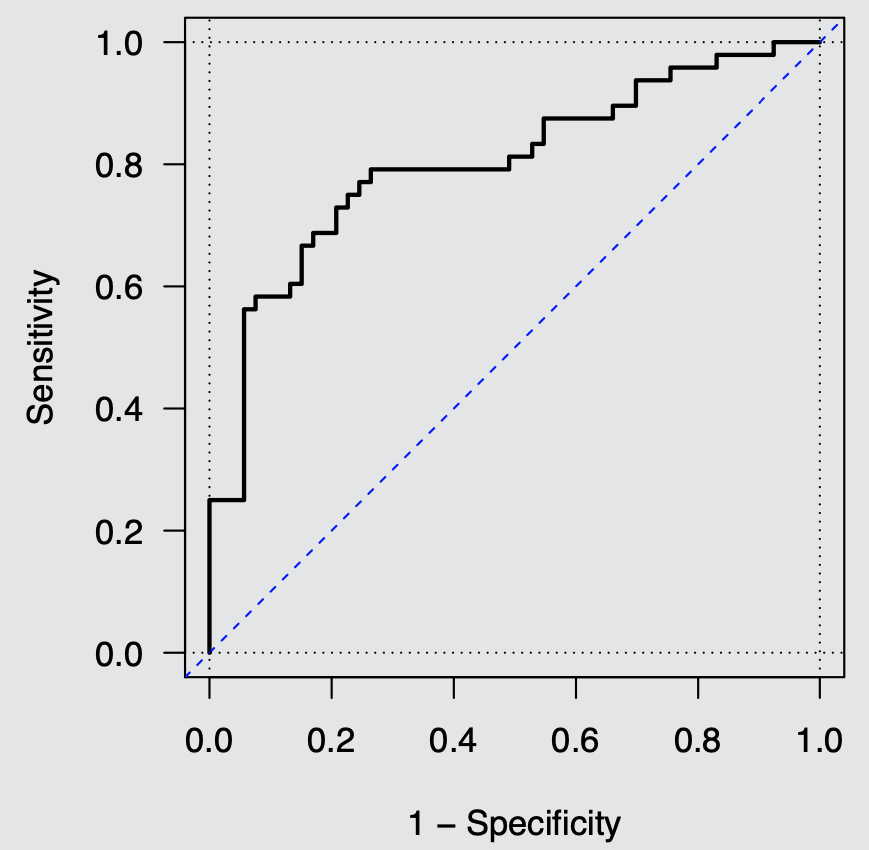
\includegraphics[scale=0.25]{ROC.png}
    \caption{Example of ROC}
    \label{}
\end{figure}\end{center}
Note: ROC curve
\begin{enumerate}[$\bullet$]
    \item is non-decreasing
    \item goes from $(0, 0)$ to $(1, 1)$
    \item is often above the $45^\circ$ line (which represents random guessing.)
    \item indicates a better classifier if it is higher
\end{enumerate}
The area under the ROC curve, a.k.a. the \textbf{“concordance index,”} \underline{measures predictive power}.


\section{Cochran-Mantel-Haenszel Tests for Common Odds Ratios}
Consider an $X-Y$ relationship as in a $2 \times 2$ table:
\begin{enumerate}[-]
    \item e.g., $\quad X=$ exposure (yes, no), $\quad Y=$ disease presence
    \item e.g., $\quad X=$ treatment $(\mathrm{A}$ or $\mathrm{B}), \quad Y=$ whether successful
\end{enumerate}
Suppose we also have a categorical \textbf{stratification variable $Z$} that might affect inference about the $X-Y$ relationship:
\begin{enumerate}[-]
    \item e.g., $\quad Z=$ age range
    \item e.g., $\quad Z=$ treatment clinic
\end{enumerate}
$Z$ could be a confounding variable, for which we want to adjust when assessing the $X-Y$ relationship.\\
If $Z$ has $K$ categories (\textbf{strata}), the data form a $2 \times 2 \times K$ contingency table.

\subsection{Model-Based: Logistic Regression}
Homogeneous association model:
$$
\begin{aligned}
& \operatorname{logit}\left(\pi_{i k}\right)=\alpha+\beta x_i+\beta_k^Z \quad i=1,2 \quad k=1, \ldots, K \\
& \pi_{i k}=\mathrm{P}(Y=1 \mid X=i, Z=k), \quad x_i=\left\{\begin{matrix}
    1 & i=1 \\
    0 & i=2
\end{matrix}\right.
\end{aligned}
$$
(For identifiability, set, e.g., $\beta_1^Z \equiv 0$).

Testing conditional independence is the same as testing
$$
H_0: \beta=0
$$
which can be done with Wald, likelihood-ratio, or score.

The common conditional odds ratio is
$$
\theta_{X Y(k)}=e^\beta \quad(\text {all } k)
$$
for which the MLE is
$$e^{\hat{\beta}}$$
Can also form a $\mathrm{Cl}$ (with Wald or profile likelihood).

Recall, this model \textit{assumes} homogeneous $XY$ association over $Z$. With grouped data, this assumption may be tested by comparison with the saturated model (e.g., using it as the full model in a LRT). (If homogeneous association is rejected, it may be worthwhile to investigate how $XY$ association varies between strata.)

\subsection{Non-Model-Based: CMH}
Consider the $k$ th partial table:
$$
\begin{array}{c|c|c|c}
\multicolumn{1}{r}{Z=k:} &\multicolumn{1}{c}{Y=1} &\multicolumn{1}{c}{Y=0}\\
\cline { 2 - 3 }
\multicolumn{1}{r|}{$X=1$} & n_{11k} & n_{12k} & n_{1+k} \\
\cline { 2 - 3 } 
\multicolumn{1}{r|}{$X=0$} & n_{21k} & n_{22k} & n_{2+k} \\
\cline { 2 - 3 } \multicolumn{1}{c}{}&\multicolumn{1}{c}{n_{+1k}}&\multicolumn{1}{c}{n_{+2k}}&\multicolumn{1}{c}{n_{++k}}
\end{array}
$$
so that
$$
n_{i j k}=\text { count in row } i \& \text { col } j \text { of table } k
$$

Suppose there is no $X Y$ association when $Z=k$.

Then conditioning on the $k$ th partial table's marginal totals (as in Fisher's exact test) yields
$$
\begin{gathered}
\mu_{11 k}=E\left(N_{11 k}\right)=\frac{n_{1+k} n_{+1 k}}{n_{++k}} \\
\operatorname{var}\left(N_{11 k}\right)=\frac{n_{1+k} n_{2+k} n_{+1 k} n_{+2 k}}{n_{++k}^2\left(n_{++k}-1\right)}
\end{gathered}
$$
based on the hypergeometric distribution.

\begin{definition}
\normalfont
Define the \textbf{(Cochran-) Mantel-Haenszel statistic}
$$
\mathrm{CMH}=\frac{\left(\sum_k\left(n_{11 k}-\mu_{11 k}\right)\right)^2}{\sum_k \operatorname{var}\left(N_{11 k}\right)}
$$
\end{definition}
Under
\begin{center}
    $H_0$ : conditional $X-Y$ independence
\end{center}
for large samples,
$$
\mathrm{CMH} \quad \dot{\sim} \quad \chi_1^2
$$
Note: If $\theta_{X Y(k)}>1$ then $n_{11 k}-\mu_{11 k}$ tends to be positive. If this is true for all $k, \mathrm{CMH}$ will tend to be larger. (Likewise if $\theta_{X Y(k)}<1$ for all $k$.) Thus reject
\begin{center}
    $H_0$ : conditional $X-Y$ independence
\end{center}
if $\mathrm{CMH}>\chi_1^2(\alpha)$.

For estimating the (common) conditional odds ratio, Mantel \& Haenszel proposed
$$
\hat{\theta}_{\mathrm{MH}}=\frac{\sum_k n_{11 k} n_{22 k} / n_{++k}}{\sum_k n_{12 k} n_{21 k} / n_{++k}}
$$
\textbf{Remark:} Even if homogeneous XY association is not exactly correct, the CMH test and $\hat{\theta}_{\mathrm{MH}}$ still serve a summary of association, especially if all true associations have the same direction.

\textbf{Remark:} In the model
$$
\operatorname{logit}\left(\pi_{i k}\right)=\alpha+\beta x_i+\beta_k^Z
$$
the condition
$$
\beta_k^Z=0 \quad \text { all } k
$$
is equivalent to conditional independence of $Y$ and $Z$ given $X$.
In that case, the conditional and marginal $X-Y$ odds ratios are the same.


\section{Existence of the MLE in Logistic Regression}
The logistic regression MLE is unique if it exists (since the log-likelihood is strictly concave when $\boldsymbol{X}$ has full rank). But it doesn't always exist ...

For simplicity, assume binary $Y$ (ungrouped data), so that $y_i=0 \text { or } 1$. Let $\boldsymbol{x}_i^T=i \text { th row of } \boldsymbol{X}$.

Technically, the logistic regression MLE exists and is unique \textbf{if and only if} there \underline{does not exist} $\boldsymbol{b} \neq \mathbf{0}$ such that, for all $i$,
$$
\begin{array}{rlr}
    \boldsymbol{b}^T \boldsymbol{x}_i>0 & \Rightarrow & y_i=1 \\
    \boldsymbol{b}^T \boldsymbol{x}_i<0 & \Rightarrow & y_i=0
\end{array}
$$
If $\boldsymbol{X}$ has full rank, then existence of the $\boldsymbol{b}$ above implies that an MLE does not exist. There is no maximum. The MLE fails to exist because the likelihood keeps increasing as \underline{one or more parameters become infinite}.

One special case when the MLE does not exist:
\begin{center}\begin{figure}[htbp]
    \centering
    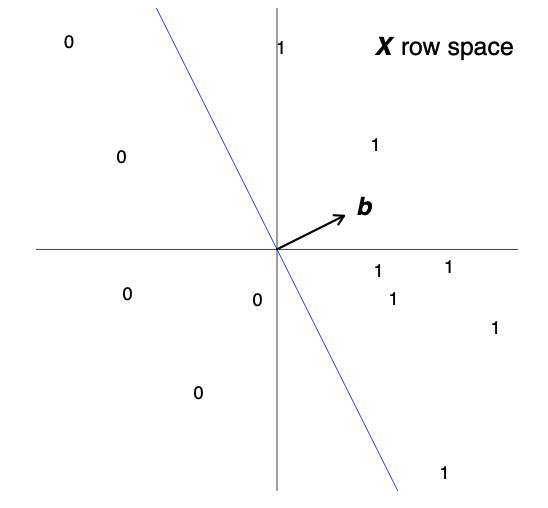
\includegraphics[scale=0.3]{complete separation.png}
    \caption{Complete Separation}
    \label{}
\end{figure}\end{center}
\begin{definition}[complete separation]
\normalfont
There exists $\boldsymbol{b} \neq \mathbf{0}$ such that, for all $i$,
$$
\begin{array}{rlr}
    y_i=1 & \Rightarrow & \boldsymbol{b}^T \boldsymbol{x}_i>0\\
    y_i=0 & \Rightarrow & \boldsymbol{b}^T \boldsymbol{x}_i<0
\end{array}
$$
i.e., a subspace separates the rows of $\boldsymbol{X}$ with $Y = 1$ from those with $Y = 0$ ...
\end{definition}
Even when complete separation does not hold, the MLE may still fail to exist.
\begin{center}\begin{figure}[htbp]
    \centering
    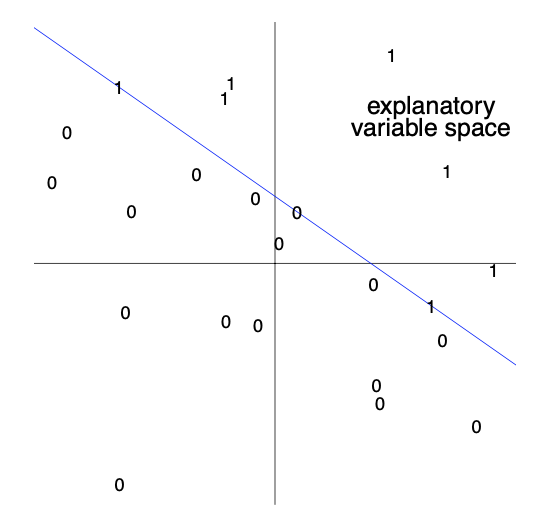
\includegraphics[scale=0.3]{quasi-complete separation.png}
    \caption{Quasi-Complete Separation}
    \label{}
\end{figure}\end{center}
\begin{definition}[quasi-complete separation]
\normalfont
Assuming the logistic regression has an intercept, \textbf{quasi-complete separation} is when a \textit{hyperplane in explanatory variable space} separates $Y = 0$ and $Y = 1$ cases, except that both cases exist on the hyperplane itself.
\end{definition}
\begin{example}
    One common situation can cause quasi-complete separation: One category of a nominal explanatory variable has only $Y =0$ cases or only $Y =1$ cases. For example, suppose $X$ is type of treatment and $Y = 1$ means cured. Then quasi-complete separation usually occurs if one treatment type cures (or fails to cure) all of its cases.
\end{example}
An MLE fails to exist under quasi-complete separation. As with complete separation, quasi-complete separation allows the likelihood to keep increasing as \underline{one or more parameters become infinite}.

\subsubsection*{Signs the MLE may not exist:}
\begin{enumerate}[1.]
    \item Numerical estimates have large magnitude.
    \item Standard errors are huge ($z$-values near $0$, P-values near $1$)
    \item Some fitted values ($\hat{\pi}_i$) are almost exactly $0$ or $1$.
    \item Iteration count is unusually large (or there is a non-convergence warning)
\end{enumerate}

\subsubsection*{Possible remedies:}
\begin{enumerate}[1.]
    \item Use likelihood-ratio or score inference (not Wald)
    \item Use alternative estimation techniques (e.g., penalized likelihood, Bayes)
    \item Use alternative fitting approaches like exact logistic regression (R packages \textit{elrm} and \textit{logistiX})
    \item Use the bias reduction method of Firth (1993) (R package \textit{brglm})
\end{enumerate}




\chapter{Multinomial Regression Models}
In this chapter we consider the situation that there are more than two categories of the response $Y$.

\section{Settings}
Suppose response $Y$ is categorical, with $J$ possible categories. The response can be
\begin{enumerate}[$\bullet$]
    \item \textbf{Nominal}. e.g. favorite soft drink (Coke, Pepsi, other)
    \item \textbf{Ordinal}. e.g. customer rating of service (good, neutral, bad)
\end{enumerate}
Let categories be coded as $1, 2, . . . , J$ (in order, if ordinal).

\subsection{Goal}
\textbf{Goal:} Model the distribution of $Y$ in terms of explanatory variables $\boldsymbol{x}=X_1,...,X_p$.

That is, we want to predict
$$
\pi_j(\boldsymbol{x})=\mathrm{P}(Y \text { in category } j \mid \boldsymbol{x}) \quad j=1, \ldots, J
$$
where $\sum_{j=1}^J \pi_j(\boldsymbol{x})=1$ for any $\boldsymbol{x}$

There are $N$ observations of $(\boldsymbol{x},Y)$. The observations of $Y$ are independent (conditional on $\boldsymbol{x}$). Use $\boldsymbol{x}_i$ to denote the explanatory vector for observation $i$.

\subsection{Formats for Multinomial Response Data}
\begin{enumerate}[$\bullet$]
    \item \textbf{Ungrouped codes:} $y_i=j$, $j\in\{1,...,J\}$.
    \item \textbf{Ungrouped indicator vectors:} $\boldsymbol{y}_i=(y_{i1},...,y_{iJ})$ where $$y_{ij}=\left\{\begin{matrix}
        1,&\textnormal{ if obs. $i$ in category $j$}\\
        0,&\textnormal{ otherwise}
    \end{matrix}\right.$$
    Then $\sum_{j=1}^J y_{ij}=1,\forall i$ and $\boldsymbol{Y}_i\sim \textnormal{multinomial}(1,\boldsymbol{\pi}(\boldsymbol{x}_i))$ where $\boldsymbol{\pi}(\boldsymbol{x})=\left(\pi_1(\boldsymbol{x}),...,\pi_J(\boldsymbol{x})\right)$.
    \item \textbf{Grouped:} Assume observation $i$ represents $n_i$ independent responses having the same explanatory vector $\boldsymbol{x}_i$ (i.e., replicates). Let $\boldsymbol{y}_i=(y_{i1},...,y_{iJ})$ where $$y_{ij}=\textnormal{number of responses in category $j$ (for obs. $i$)}$$
    Then $\sum_{j=1}^J y_{ij}=n_i$ and $\boldsymbol{Y}_i\sim \textnormal{multinomial}(n_i,\boldsymbol{\pi}(\boldsymbol{x}_i))$\\
    Parametric models assume a form for each $\pi_j(\boldsymbol{x})$ in terms of (vector) parameter $\boldsymbol{\theta}$.\\
    The likelihood:
    $$
    \ell(\boldsymbol{\theta}) \propto \prod_{i=1}^N \prod_{j=1}^J \pi_j\left(\boldsymbol{x}_i ; \boldsymbol{\theta}\right)^{y_{i j}}
    $$
    where $y_{i j}$ is from the ungrouped indicator or grouped format.
\end{enumerate}


\section{Nominal Responses}
\subsection{Baseline-Category Logistic Model}
For the response whose categories are nominal, we can consider a \textbf{baseline-category logistic model}.
\begin{definition}[Baseline-Category Logistic Model]
    \normalfont
    The \textbf{baseline-category logistic model}:
    \begin{equation}
        \begin{aligned}
            \ln\left(\frac{\pi_{j}(\boldsymbol{x})}{\pi_J(\boldsymbol{x})}\right)=\alpha_j+\boldsymbol{\beta}_j^T \boldsymbol{x},\quad j=1,...,J-1
        \end{aligned}
        \nonumber
    \end{equation}
    These are the \textbf{baseline (category) logits}, with $J$ as the \textbf{baseline category}.\\
    The $J-1$ values of $\alpha_j$ and $J-1$ vectors $\boldsymbol{\beta}_j$ are unrestricted parameters to be estimated (MLE).\\
    For the sake of notation, also define $\alpha_J\equiv0$ and $\boldsymbol{\beta}_J\equiv \boldsymbol{0}$
\end{definition}
Logits for other pairs of categories can also be determined: For categories $a$ and $b$,
\begin{equation}
    \begin{aligned}
        \ln\left(\frac{\pi_{a}(\boldsymbol{x})}{\pi_b(\boldsymbol{x})}\right)&=\ln\left(\frac{\pi_{a}(\boldsymbol{x})}{\pi_J(\boldsymbol{x})}\right)-\ln\left(\frac{\pi_{b}(\boldsymbol{x})}{\pi_J(\boldsymbol{x})}\right)\\
        &=(\alpha_a-\alpha_b)+(\boldsymbol{\beta}_a-\boldsymbol{\beta}_b)^T \boldsymbol{x}
    \end{aligned}
    \nonumber
\end{equation}

Based on the model, we have
\begin{equation}
    \begin{aligned}
        \frac{\pi_{j}(\boldsymbol{x})}{\pi_J(\boldsymbol{x})}=e^{\alpha_j+\boldsymbol{\beta}_j^T \boldsymbol{x}}
    \end{aligned}
    \nonumber
\end{equation}
Solving (using that the probabilities sum to $1$) gives
\begin{equation}
    \begin{aligned}
        \pi_{j}(\boldsymbol{x})=\frac{e^{\alpha_j+\boldsymbol{\beta}_j^T \boldsymbol{x}}}{\sum_{h=1}^J e^{\alpha_h+\boldsymbol{\beta}_h^T \boldsymbol{x}}}
    \end{aligned}
    \nonumber
\end{equation}
recalling that $\alpha_J\equiv0$ and $\boldsymbol{\beta}_J\equiv \boldsymbol{0}$.

Remark: Unlike in the binomial case, $ \pi_{j}(\boldsymbol{x})$ is not necessarily a monotone function of each $X$ variable.

\subsubsection*{Interpretation}
Suppose there is just one explanatory variable $X$ (quantitative or indicator).

Then we call $\frac{\pi_{j}(x)}{\pi_J(x)}=e^{\alpha_j+\beta_j x}$ \underline{the odds of $j$ relative to $J$}.

Then, $e^{\beta_j}$ is the multiplicative change in this odds when $X$ increases by $1$.

\subsubsection*{Estimation}
We consider MLEs
\begin{equation}
    \begin{aligned}
        \hat{\alpha}_1,...,\hat{\alpha}_{J-1}, \hat{\boldsymbol{\beta}}_1,...,\hat{\boldsymbol{\beta}}_{J-1}
    \end{aligned}
    \nonumber
\end{equation}
(when they uniquely exist).\\
\textbf{Note:} The total number of (scalar) free parameters is $(J-1)(1+p)$, where $\boldsymbol{x}$ has $p$ elements. The (residual) degrees of freedom depends on the data format —-- grouped data with N multinomial observations generally have $(J-1)(N-(1+p))$ degrees of freedom (df).\\
Substituting the MLEs gives estimated response functions $$\hat{\pi}_j(\boldsymbol{x}),\forall j$$, "fitted values" $$\hat{\pi}_{ij}=\hat{\pi}_j(\boldsymbol{x}_i),\forall i,j$$, and estimated logits, such as $$\ln\left(\frac{\hat{\pi}_{j}(\boldsymbol{x})}{\hat{\pi}_J(\boldsymbol{x})}\right)=\hat{\alpha}_j+\hat{\boldsymbol{\beta}}_j^T\boldsymbol{x}$$

\section{Ordinal Responses}
Let response $Y$ be ordinal, ungrouped, and represented with codes $1,2,...,J$ in that order.

Note: $P(Y\leq j\mid \boldsymbol{x})=\pi_1(\boldsymbol{x})+\cdots+\pi_j(\boldsymbol{x}),\ j=1,...,J$

\subsection*{Proportional Odds Model}
The \textbf{cumulative logits} are
\begin{equation}
    \begin{aligned}
        \textnormal{logit}\left(P(Y\leq j\mid \boldsymbol{x})\right)=\ln\left(\frac{P(Y\leq j\mid \boldsymbol{x})}{P(Y> j\mid \boldsymbol{x})}\right),\quad j=1,...,J-1
    \end{aligned}
    \nonumber
\end{equation}

\begin{definition}[Proportional Odds Model]
    \normalfont
    The \textbf{proportional odds model:}
    \begin{equation}
        \begin{aligned}
            &\textnormal{logit}\left(P(Y\leq j\mid \boldsymbol{x})\right)=\alpha_j+\boldsymbol{\beta}^T \boldsymbol{x},\\
            &j=1,...,J-1,\quad \alpha_1\leq\alpha_2\leq\cdots\leq\alpha_{J-1}
        \end{aligned}
        \nonumber
    \end{equation}
    Note:
    \begin{enumerate}[$\bullet$]
        \item For each $j$, this is a logistic regression, with \textbf{binary outcome} indicating subset $\{1, . . . , j\}$ versus $\{j + 1, . . . , J\}$.
        \item $\boldsymbol{\beta}$ does not depend on $j$.
    \end{enumerate}
\end{definition}
The order restriction on the $\alpha_j$ values is induced by the increasing property of logit function. As $0<P(Y\leq j\mid \boldsymbol{x})\leq P(Y\leq j+1\mid \boldsymbol{x})<1$, the logit is increasing $0\leq \textnormal{logit}\left(P(Y\leq j+1\mid \boldsymbol{x})\right)-\textnormal{logit}\left(P(Y\leq j\mid \boldsymbol{x})\right)=\alpha_{j+1}-\alpha_j$.

We use the differenece of $\alpha_j$ to represent the different of cumularive probaility for different $j$, and fixing the $\boldsymbol{\beta}$ for all $j$ to avoid the wrong order.

The probabilities $\pi_j(\boldsymbol{x})$ can be recovered from the cumulative probabilities:
\begin{equation}
    \begin{aligned}
        \pi_j(\boldsymbol{x})=\left\{\begin{matrix}
            P(Y\leq 1\mid \boldsymbol{x}),&j=1\\
            P(Y\leq j\mid \boldsymbol{x})-P(Y\leq j-1\mid \boldsymbol{x}),&1<j<J\\
            1-P(Y\leq J-1\mid \boldsymbol{x}),&j=J
        \end{matrix}\right.
    \end{aligned}
    \nonumber
\end{equation}

\subsubsection*{Interpretation: Proportional Odds}
For some $j<J$, consider the cumulative odds ratio
\begin{equation}
    \begin{aligned}
        \frac{\textnormal{odds}(Y\leq j\mid \boldsymbol{x}_1)}{\textnormal{odds}(Y\leq j\mid \boldsymbol{x}_2)}
    \end{aligned}
    \nonumber
\end{equation}
i.e., the odds ratio for $Y \leq j$ at $\boldsymbol{x}_1$ versus $\boldsymbol{x}_2$.\\
Its natural logarithm is
$$
\begin{aligned}
& \operatorname{logit}\left(\mathrm{P}\left(Y \leq j \mid \boldsymbol{x}_1\right)\right)-\operatorname{logit}\left(\mathrm{P}\left(Y \leq j \mid \boldsymbol{x}_2\right)\right) \\
&=\left(\alpha_j+\boldsymbol{\beta}^T \boldsymbol{x}_1\right)-\left(\alpha_j+\boldsymbol{\beta}^T \boldsymbol{x}_2\right) \\
&=\boldsymbol{\beta}^T\left(\boldsymbol{x}_1-\boldsymbol{x}_2\right)
\end{aligned}
$$
which does not depend on $j$.

When $p = 1$, the log cumulative odds ratio becomes $\beta (x_1-x_2)$, which is proportional to $x_1-x_2$, with the same proportionality constant for all $j$.

If $x_1-x_2=1$, the cumulative odds ratio (for any $j<J$) is $e^\beta$, which should be independent to $j$.

\begin{example}
    Consider the implications when $X$ is binary and $J = 3$:
    \begin{center}
        \begin{tabular}{rccccc}
        \multicolumn{1}{r}{}&\multicolumn{2}{c}{$Y=1$}&\multicolumn{2}{c}{$Y=2$}&\multicolumn{1}{c}{$Y=3$}\\
        \cline{2-6}
        \multicolumn{1}{r|}{$X=1$}&\multicolumn{2}{c|}{$\pi_1(1)$}&\multicolumn{2}{c|}{$\pi_2(1)$}&\multicolumn{1}{c|}{$\pi_3(1)$}\\
        \cline{2-6}
        \multicolumn{1}{r|}{$X=0$}&\multicolumn{2}{c|}{$\pi_1(0)$}&\multicolumn{2}{c|}{$\pi_2(0)$}&\multicolumn{1}{c|}{$\pi_3(0)$}\\
        \cline{2-6}
        \multicolumn{1}{c}{}&&&&&
        \end{tabular}
    \end{center}
    with rows sum to $1$.\\
    Under the proportional odds model, we must have
    \begin{equation}
        \begin{aligned}
            e^\beta=\frac{\pi_1(1)(\pi_2(0)+\pi_3(0))}{(\pi_2(1)+\pi_3(1))\pi_1(0)}=\frac{(\pi_1(1)+\pi_2(1))\pi_3(0)}{\pi_3(1)(\pi_1(0)+\pi_2(0))}
        \end{aligned}
        \nonumber
    \end{equation}
\end{example}

\subsubsection*{Checking the Proportional Odds Assumption}
Can use a test (e.g. LRT) of the fitted model versus a more general model that allows a separate $\boldsymbol{\beta}_j$ for each cumulative logit ($j = 1, . . . , J - 1$).

(The more general model allows non-parallel curves, leading to possibly invalid probabilities. But it might still fit adequately within the range of the data.)

\subsubsection*{Model Fitting}
Usually by maximum likelihood (Fisher scoring or Newton-Raphson).



\subsection{Latent Variable Formulation}
Besides proportional odds, what other models are available?
\begin{definition}[Latent Variable Formulation]
    \normalfont
    Suppose $Y$ derives from a latent continuous variable $Y^*$:
    \begin{center}\begin{figure}[htbp]
        \centering
        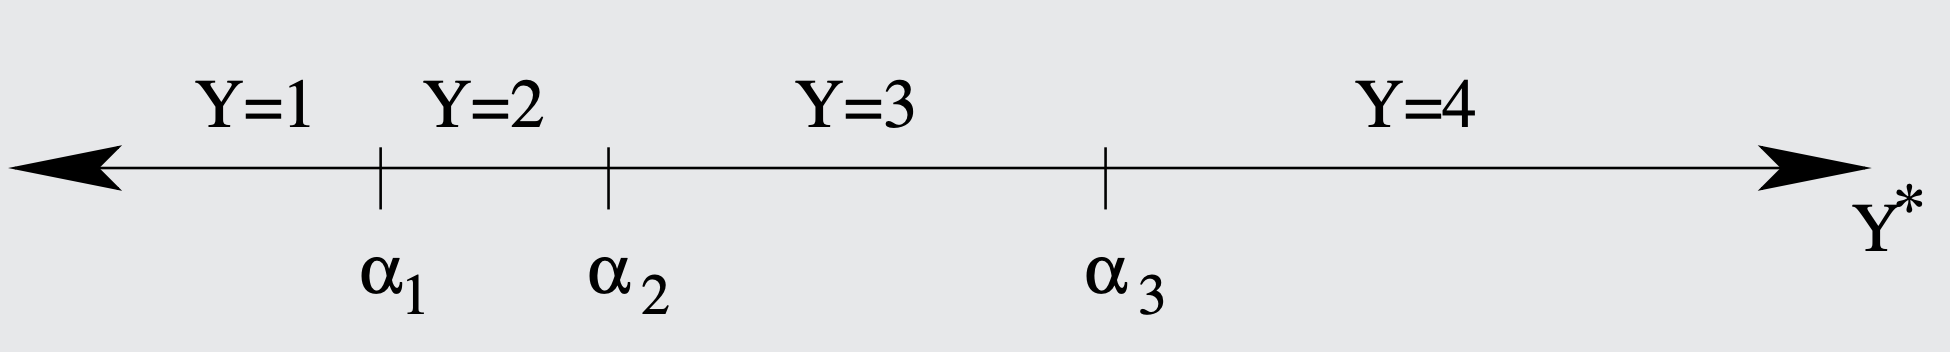
\includegraphics[scale=0.5]{LVF.png}
        \caption{The real line is divided into $J$ successive segments (with unknown boundaries), and $Y$ indicates which one contains $Y^*$.}
        \label{}
    \end{figure}\end{center}
\end{definition}



























































\end{document}